\documentclass[a4paper]{article}
\usepackage[spanish,activeacute]{babel}
\usepackage[ansinew]{inputenc}
\usepackage{cite}
% Anda fen'omeno mientras codifiquemos el archivo como ansi.
\usepackage{graphicx}
\usepackage[left=2cm,right=2cm]{geometry}
\usepackage{ulem} %Para tachar cosas
\usepackage{epigraph}
\usepackage{listings}
\usepackage{html}
\usepackage{booktabs}
\usepackage[colorlinks=true]{hyperref}
\bibliographystyle{plainurl}
\parindent = 0 pt
\parskip = 11 pt

\newcommand{\haskell}{\textsl{Haskell}}
\newcommand{\hpage}{\textbf{\textsl{$\lambda$Page}}}
\newcommand{\cabal}{\textsl{Cabal}}

\begin{document}

    \thispagestyle{empty}
    \begin{center}
	    {\Large Tesis de Licenciatura}\\[1em]
	    {\huge \textbf{$\lambda$Page}}\\[0.5em]
	    {\large \textit{Un bloc de notas para desarrolladores Haskell}}\\[1em]
	    \par\vspace{\stretch{1}}
	    {\large Departamento de Computaci\'on}\\[0.5em]
	    {\large Facultad de Ciencias Exactas y Naturales}\\[0.5em]
	    {\large Universidad de Buenos Aires}
	    \par\vspace{\stretch{1}}
	    \begin{figure}[h]
	        \begin{center}
	        
\includegraphics[width=40mm]{pictures/logoUba}
	        \end{center}
	    \end{figure}
	    {\Large \textbf{Alumno}}\\[0.8em]
	    {\Large Fernando Benavides (LU 470/01)} \par
	    {\Large greenmellon@gmail.com} \par
	    \par\vspace{\stretch{1}}
	    {\Large \textbf{Directores}}\\[0.8em]
	    {\Large Dr. Diego Garbervetsky} \par
	    {\Large Lic. Daniel Gor'in} \par
	    \par\vspace{\stretch{2}}
         {\Large \textbf{Abstract}}\\[0.5em]
    \end{center}
    El presente documento describe una herramienta para desarrolladores \haskell\ que pretende facilitar la tarea de ``debuggear'', analizar y entender c'odigo, llamada \hpage.  Con ella el usuario puede manipular ``p'aginas'' de texto libre que contengan expresiones \haskell, intentar interpretar 'estas expresiones independientemente y analizar los resultados obtenidos.
    \vspace*{\stretch{3}}
    \newpage

\tableofcontents

\newpage
\section{Estructura del Informe}
\paragraph{}El presente informe pretende presentar a \hpage, una herramienta para facilitar el trabajo de los desarrolladores \haskell.  El mismo se encuentra dividido en cuatro secciones.
\paragraph{}La primera es una secci'on en la que describiremos los motivos que nos llevaron a desarrollar esta herramienta, hablaremos tambi'en de otras herramientas similares y presentaremos \hpage\ de modo general, mostrando principalmente el lugar que pretendemos que ocupe dentro del mundo \haskell.
\paragraph{}En la siguiente secci'on intetaremos mostrar, a trav'es de dos tutoriales, c'omo utilizar \hpage\ y daremos a conocer sus virtudes y capacidades.  Para comenzar, aprenderemos c'omo instalarlo, de modo que el lector pueda, una vez instalado el sistema, seguir los tutoriales paso a paso y realizar sus propias experiencias.
\subparagraph{}Luego, presentaremos un tutorial destinado al p'ublico ``acad'emico'' que nos mostrar'a c'omo utilizar la herramienta para resolver ejercicios pr'acticos t'ipicos de varias materias de la facultad.  Veremos all'i la facilidad de trabajo que brinda \hpage\ al alumno permiti'endole descubrir paso a paso el lenguaje y sus caracter'isticas principales.
\subparagraph{}El segundo tutorial que presentaremos est'a apuntado a aquellos desarrolladores que trabajan con proyectos \haskell\ de dimensiones mayores a lo visto en el 'ambito acad'emico.  La idea de este tutorial es mostrar c'omo \hpage\ puede ayudarlos a entender c'odigo existente y tambi'en a generar y testear nuevo c'odigo de manera sencilla y veloz.
\paragraph{}Una vez observado \hpage\ en funcionamiento y destacadas sus caracter'isticas principales, observaremos c'omo ha sido dise'nado y constru'ido.  Podremos ver los requerimientos que guiaron su dise'no, la arquitectura conceptual que lo subyace y las principales decisiones de dise'no e implementaci'on que se han tomado durante su desarrollo.
\paragraph{}Finalmente observaremos los resultados obtenidos y los contrastaremos con los objetivos planteados al inicio de este desarrollo.  Estableceremos el estado del proyecto en general, cu'ales son los siguientes pasos a dar y qu'e otras tareas pueden llevarse a cabo a partir de ahora.

\newpage
\section{Introducci'on}
\subsection{Motivaci'on}
\begin{epigraphs}
    \qitem{Motivation is what gets you started. Habit is what keeps you going}{Jim Rohn}
    \qitem{Essstamo mo-ti-va-do, nene}{El ``Bambino'' Veira}
\end{epigraphs}
\paragraph{}Actualmente estamos presenciando un importante cambio en el desarrollo de sistemas, gracias al 'exito de proyectos como \htmladdnormallink{CouchDB}{http://couchdb.apache.org}~\cite{couchdb}, \htmladdnormallink{ejabberd}{http://www.ejabberd.im}~\cite{ejabberd} y el chat de \htmladdnormallink{Facebook}{http://www.facebook.com/}~\cite{facebook}, todos ellos desarrollados utilizando lenguajes del paradigma funcional.
\paragraph{}Ejemplos de 'estos lenguajes de programaci'on, como \htmladdnormallink{Haskell}{http://www.haskell.org}~\cite{haskell} o \htmladdnormallink{Erlang}{http://www.erlang.org}~\cite{erlang}, demuestran ser maduros, confiables y presentan claras ventajas en comparaci'on con los lenguajes tradicionales del paradigma imperativo.  Sin embargo, los desarrolladores que deciden realizar el cambio de paradigma se encuentran con el problema de la escasez de ciertas herramientas que les permitan realizar su trabajo m'as eficientemente.  Por el contrario, 'estas herramientas abundan en el desarrollo de proyectos utilizando lenguajes orientados a objetos.  En particular, nuestro foco de atenci'on se centra sobre aquellas herramientas que permiten realizar \textsl{debugging} y \textsl{entendimiento} de c'odigo a trav'es de \textsl{``micro-testing''}\footnote{Enti'endase \textsl{micro-testing} como la tarea de realizar tests eventuales para entender o evaluar alg'un aspecto de un programa} .
\paragraph{}Los desarrolladores Haskell cuentan actualmente con dos herramientas de este tipo:
\begin{description}
	\item[\htmladdnormallink{GHCi}{http://www.haskell.org/ghc/docs/latest/html/users\_guide/ghci.html}~\cite{ghci}]
		La consola que provee \htmladdnormallink{GHC}{http://www.haskell.org/ghc}~\cite{ghc} permite a los desarrolladores evaluar expresiones, verificar su tipo o su clase.  Cuenta tambi'en con un \htmladdnormallink{mecanismo de debugging}{http://www.haskell.org/ghc/docs/6.10-latest/html/users\_guide/ghci-debugger.html}~\cite{ghcdebug} integrado que permite realizar la evaluaci'on de expresiones paso a paso.  Pese a ser la herramienta m'as utilizada por los desarrolladores, \textit{GHCi} tiene varias limitaciones.  En particular:
		\begin{itemize}
			\item No permite editar m'as de una expresi'on a la vez
			\item No permite intercalar expresiones con definiciones
			\item	Si bien permite utilizar definiciones, 'estas se pierden al recargar m'odulos
			\item No es sencillo utilizar en una sesi'on las definiciones y/o expresiones creadas en sesiones anteriores
		\end{itemize}
	\item[\htmladdnormallink{Hat}{http://www.haskell.org/hat}~\cite{hat}]
		Un herramienta para realizar seguimiento a nivel de c'odigo fuente.  A trav'es de la generaci'on de trazas de ejecuci'on, \textit{Hat} ayuda a localizar errores en los programas y es 'util para entender su funcionamiento.  Sin embargo, por estar basado en la generaci'on de trazas, requiere la compilaci'on y ejecuci'on de un programa para poder utilizarlo y esto no siempre es c'omodo para el desarrollador que puede querer simplemente analizar una expresi'on particular que incluso quiz'a no compile a'un.  Adem'as, su mantenimiento activo parece haber cesado hace m'as de un a'no y en su p'agina se observa una importante lista de problemas conocidos y caracter'isticas deseadas.
\end{description}

%%------------------------------------------------------------------------------------------------------------------------------
\subsection{Trabajos Relacionados}
\begin{epigraphs}
	\qitem{If I have seen further it is only by standing on the shoulders of giants}{Isaac Newton}
	\qitem{I like work; it fascinates me. I can sit and look at it for hours}{Jerome Klapka}
\end{epigraphs}
\paragraph{}En el mundo de la programaci'on orientada a objetos podemos encontrar herramientas como \htmladdnormallink{Java Scrapbook Pages}{http://help.eclipse.org/help33/index.jsp?topic=/org.eclipse.jdt.doc.user/reference/ref-34.htm}~\cite{javascrapbook} para \htmladdnormallink{Java}{http://www.java.com}~\cite{java} y \htmladdnormallink{Workspace}{http://wiki.squeak.org/squeak/1934}~\cite{insidesmalltalk, smalltalkworkspace} para \htmladdnormallink{SmallTalk}{http://www.smalltalk.org}~\cite{smalltalk}.  Utilizando estos aplicativos, los desarrolladores pueden introducir peque'nas porciones de c'odigo, ejecutarlas y luego inspeccionar y analizar los resultados obtenidos.  Un concepto compartido por ambas herramientas es el de presentar ``p'aginas'' de texto en las que varias expresiones pueden intercalarse con partes de texto libre y permitir al desarrollador intentar evaluar s'olo una porci'on de todo lo escrito.  Estas p'aginas pueden ser guardardas y luego recuperadas de modo de poder analizar nuevamente las mismas expresiones.  Adem'as permiten crear objetos (lo que para los lenguajes funcionales equivaldr'ia a definir expresiones) locales a la p'agina en uso y utilizarlos en ella.
\paragraph{}Dentro del paradigma funcional, con un enfoque similar, aunque un poco m'as orientado a la presentaci'on y visualizaci'on de documentos, \htmladdnormallink{Keith Hanna}{http://www.cs.kent.ac.uk/people/staff/fkh/} de la Universidad de Kent, ha desarrollado \htmladdnormallink{Vital}{http://www.cs.kent.ac.uk/projects/vital/}~\cite{vital}.  \textsl{Vital} es una implementaci'on de un entorno de visualizaci'on de documentos para \haskell.  Pretende presentar \haskell\ de una manera apropiada para usuarios finales en areas de aplicaci'on como la ingenier'ia, las matem'aticas o las finanzas.  Dentro de esta herramienta, los m'odulos \haskell\ son presentados como documentos en los que pueden visualizarse los valores que en ellos se definen directamente en el lugar en el que aparecen, ya sea de modo textual o gr'afico (como ``vistas''). 
\paragraph{}Durante el desarrollo de \hpage\ hemos tenido que enfrentar varios desaf'ios relacionados principalmente con el desarrollo de interfaces visuales dentro del paradigma funcional.  Volcando el conocimiento adquirido durante ese proceso, hemos desarrollado \htmladdnormallink{wxhNotepad}{http://github.com/elbrujohalcon/wxhnotepad}~\cite{wxhnotepad} que es, ante todo, una prueba de concepto sobre c'omo desarrollar editores de texto con \textsl{wxHaskell}.  Gracias a \htmladdnormallink{Jeremy O'Donoghue}{http://wewantarock.wordpress.com/about/}, \textsl{wxhNotepad} est'a siendo publicado como \htmladdnormallink{un tutorial}{http://wewantarock.wordpress.com/2010/01/31/building-a-text-editor-part-1/}~\cite{wewantarock} en sucesivos art'iculos en su blog
%%------------------------------------------------------------------------------------------------------------------------------
\subsection{\hpage}
\begin{epigraphs}
    \qitem{Ancorch'e lo ingegno umano faccia invenzioni varie, rispondendo con vari strumenti a un medesimo fine, mai esso trover\`a invenzione pi\`u bella, n'e pi\`u facile n'e pi\`u brieve della natura, perch'e nelle sue invenzioni nulla manca e nulla \`e superfluo}{Leonardo da Vinci}
    \qitem{La programaci'on intensiva y el uso prolongado de Tetris s'olo lleva a ver estructuras de orden y secuencias en la verduler'ia y a querer apilar los autos para formar l'ineas s'olidas}{Dar'io Ruellan}
\end{epigraphs}
\paragraph{} \htmladdnormallink{\hpage}{http://haskell.hpage.com}~\cite{hpage} se presenta como una herramienta  similar al Workspace de \textit{Smalltalk}, que permite a los desarrolladores trabajar con documentos de texto libre que incluyan expresiones y definiciones.  \hpage\ es capaz de identificar las expresiones y definiciones v'alidas y permite al desarrollador inspeccionarlas, evaluarlas, conocer su tipo y su clase.
\subparagraph{}En el esp'iritu de las herramientas provistas por la comunidad de desarrolladores \haskell, \hpage\ se integra con \htmladdnormallink{Cabal}{http://www.haskell.org/cabal}~\cite{cabal} y \htmladdnormallink{Hayoo!}{http://holumbus.fh-wedel.de/hayoo}~\cite{hayoo} y se encuentra ya disponible en \htmladdnormallink{HackageDB}{http://hackage.haskell.org/package/hpage}~\cite{hackage}.
\subparagraph{}\hpage\ presenta una interfaz simple e intuitiva, desarrollada utilizando \htmladdnormallink{wxHaskell}{http://haskell.org/haskellwiki/WxHaskell}~\cite{wxhaskell}, lo que lo convierte en una aplicaci'on multiplataforma.
\subparagraph{}Por ser una herramienta desarrollada con \haskell\ para \haskell, \hpage\ se diferencia de sus pares del mundo de objetos, al aprovechar conceptos claves como son el tipado est'atico, que permite detectar errores de tipo velozmente, evitando el costo de evaluar expresiones complejas, y la evaluaci'on perezosa, que permite evaluar expresiones infinitas e ir exhibiendo resultados progresivamente.
\subparagraph{}A diferencia de \textsl{GHCi} que es una herramienta ``de consola'', \hpage\ permite visualizar resultados de manera m'as din'amica, permitiendo que errores intermedios, detectados durante la evaluaci'on de una expresi'on no impidan continuar con la misma hasta llegar a un resultado m'as completo.
\subparagraph{}\hpage\ se encuentra desarrollado utilizando \htmladdnormallink{\textsl{eprocess}}{http://hackage.haskell.org/package/eprocess}~\cite{eprocess}, una librer'ia que facilita el manejo de ``threads'' en un estilo similar al de los procesos \textsl{Erlang}.  Gracias al uso de esta librer'ia, \hpage\ puede realizar tareas en paralelo y por lo tanto permitir al usuario continuar editando los documentos en los que est'a trabajando mientras espera que se eval'ue una expresi'on e incluso cancelar una evaluaci'on conservando la porci'on del resultado obtenida hasta ese momento.  Tambi'en gracias al uso de \textsl{eprocess}, \hpage\ permite detectar c'alculos infinitos e informar sobre este hecho al usuario para que ya no siga esperando indefinidamente el resultado de la evaluaci'on solicitada.
\newpage

\section{Descubriendo \hpage}
\subsection{Instalaci'on}
\begin{epigraphs}
	\qitem{As a rule, software systems do not work well until they have been used, and have failed repeatedly, in real applications.}{Dave Parnas}
	\qitem{The \#1 programmer excuse for legitimately slacking off: ``My code is compiling''}{David Knutz}
\end{epigraphs}
\paragraph{}Para instalar \hpage\ en \textsl{OSX} o \textsl{Windows}, se proveen instaladores en el sitio web de \hpage, pero, como ya se ha dicho, \hpage\ se encuentra en \textsl{HackageDB} y por lo tanto el modo oficial de instalarlo es utilizando \cabal, con el siguiente comando:
\lstset{language=sh, frame=single, tabsize=2}
\begin{center}\begin{lstlisting}
$ cabal install hpage
\end{lstlisting}\end{center}
\subparagraph{}Sin embargo, para ello, previamente se deben satisfacer las siguientes dependencias:
\begin{description}
	\item[\htmladdnormallink{wxWidgets 2.8.10+}{http://www.wxwidgets.org/downloads/}~\cite{wxwidgets}] El framework de desarrollo para interfaces de usuario que utiliza \textsl{wxHaskell}.  Debe ser instalado con los m'odulos unicode, cmdline, config, log, stl, richtext y clipboard, al menos y con el m'odulo odbc desactivado.
	\item[\htmladdnormallink{Haskell Platform}{http://hackage.haskell.org/platform/}~\cite{platform}] Una distribuci'on de \haskell\ que incluye todo lo necesario para compilar e instalar programas desarrollados en este lenguaje (de particular inter'es para \hpage: GHC y happy).
\end{description}
\subsubsection{Windows}
\paragraph{}Para el correcto funcionamiento de \hpage\ los usuarios de \textsl{Windows XP} deben instalar el \htmladdnormallink{C++ 2008 SP1}{http://www.microsoft.com/downloads/details.aspx?familyid=A5C84275-3B97-4AB7-A40D-3802B2AF5FC2}~\cite{cppsp1}.
\subsubsection{Linux}
\paragraph{}En algunas distribuciones de Linux es conveniente, adem'as de la instalaci'on de \textsl{Haskell Platform} instalar las librer'ias de \textit{Monad Transformers} ejecutando, por ejemplo:
\begin{center}\begin{lstlisting}
$ sudo aptitude install libghc6-mtl-dev libghc6-mtl-doc
\end{lstlisting}\end{center}
\newpage
\subsection{Caso de Uso: Aprobando PLP con \hpage}
\begin{epigraphs}
	\qitem{Es como un 'arbol, pero al rev'es: con la ra'iz abajo}{Eduardo Bonelli, profesor de PLP}
	\qitem{How is education supposed to make me feel smarter? Besides, every time I learn something new, it pushes some old stuff out of my brain - remember when I took that home winemaking course, and I forgot how to drive?}{Homer Simpons}
\end{epigraphs}
\paragraph{}Mostraremos a continuaci'on, a trav'es de un ejemplo, c'omo utilizar \hpage.  En este caso, hemos tomado prestada una pr'actica de la materia \textsl{Paradigmas de Lenguajes de Programaci'on}~\cite{plp}.  Exhibiremos entonces, c'omo un alumno podr'ia utilizar \hpage\ para resolver algunos de los ejercicios que all'i se presentan.  Seleccionamos s'olo aquellos que a nuestro criterio son los m'as representativos a la hora de entender c'omo \hpage\ ayuda al alumno en su resoluci'on.

\subsubsection{Pasos previos}
\paragraph{}Antes de comenzar a resolver los ejercicios, el alumno ejecuta \hpage\ y clickea en el bot'on \textsl{New}.  El programa presentar'a una pantalla similar a la de la figura \ref{tut100}.
\begin{figure}[hp]
	\begin{center}
        	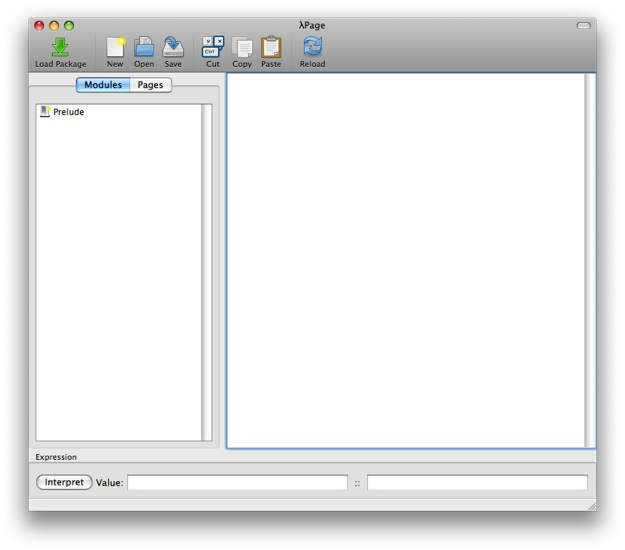
\includegraphics[width=.75\textwidth]{pictures/tut1/00}
		\caption{Tutorial 1 - Previo a comenzar}
		\label{tut100}
	\end{center}
\end{figure}

\newpage
\subsubsection{Definici'on de Tipos y Currificaci'on}
\paragraph{Ejercicio 1}Dado el siguiente programa, ?`Cu'al es el tipo de \texttt{ys}?
\lstset{language=haskell, frame=single, tabsize=4}
\begin{center}\begin{lstlisting}
	xs = [1,2,3]::[Float]
	ys = map (+) xs
\end{lstlisting}\end{center}
\subparagraph{Resoluci'on}Para resolver este ejercicio, el alumno simplemente ingresa el c'odigo provisto por la c'atedra en la p'agina de \hpage, separando ambas expresiones por un rengl'on en blanco y agregando la expresi'on de la que desea conocer el tipo (\texttt{ys}) al final.  Luego de ello, simplemente presiona el bot'on \textsl{Interpret} y puede observar el tipo del resultado (\texttt{[Float -> Float]}), tal como lo muestra la figura \ref{tut101}.
\begin{figure}[hp]
	\begin{center}
        	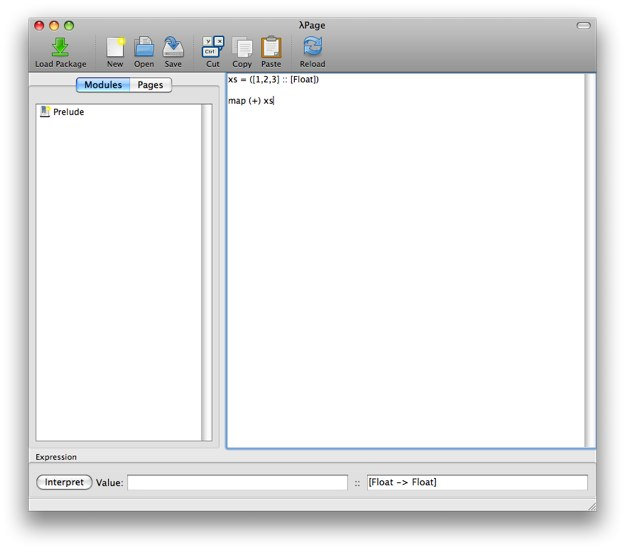
\includegraphics[width=.75\textwidth]{pictures/tut1/01}
		\caption{Tutorial 1 - Ejercicio 1}
		\label{tut101}
	\end{center}
\end{figure}

\newpage
\subsubsection{Listas por Comprensi'on}
\paragraph{Ejercicio 4}?`Cu'al es el valor de esta expresi'on?
\lstset{language=haskell, frame=single, tabsize=4}
\begin{center}\begin{lstlisting}
	[ x | x <- [1..4], y <- [x..5], (x+y) `mod` 2 == 0 ]
\end{lstlisting}\end{center}
\subparagraph{Resoluci'on}Este ejercicio se resuelve simplemente copiando y pegando el c'odigo dentro de \hpage, seleccionando la expresi'on a evaluar (si es que no se ha borrado las expresiones anteriores) y evalu'andola con el bot'on \textsl{Interpret}.  \hpage\ mostrar'a entonces el resultado: \texttt{[1,1,1,2,2,3,3,4]} como se ve en la figura \ref{tut102}.
\begin{figure}[hp]
	\begin{center}
        	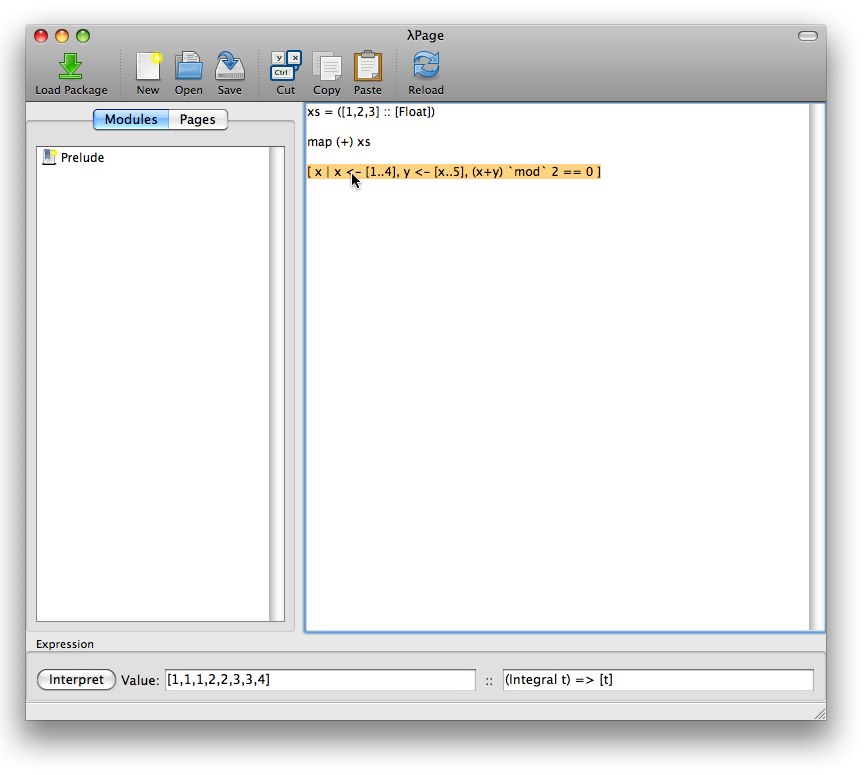
\includegraphics[width=.75\textwidth]{pictures/tut1/02}
		\caption{Tutorial 1 - Ejercicio 4}
		\label{tut102}
	\end{center}
\end{figure}

\paragraph{Ejercicio 5}Una tripla pitag'orica es una tripla $(a,b,c)$ de enteros positivos tal que $a^{2} + b^{2} = c^{2}$.  La siguiente es una definici'on de una lista (infinita) de triplas pitag'oricas.  Explicar por qu'e esta definici'on no es muy 'util.  Dar una definici'on mejor.
\begin{center}\begin{lstlisting}
	
\end{lstlisting}\end{center}
\subparagraph{Resoluci'on}Para resolver este ejercicio, el alumno podr'ia comenzar por intentar evaluar la lista que se le provee, para ello reacomodar'a su definici'on tal como se observa en la figura \ref{tut103} y presionar'a el bot'on \textsl{Interpret}.
\begin{figure}[hp]
	\begin{center}
        	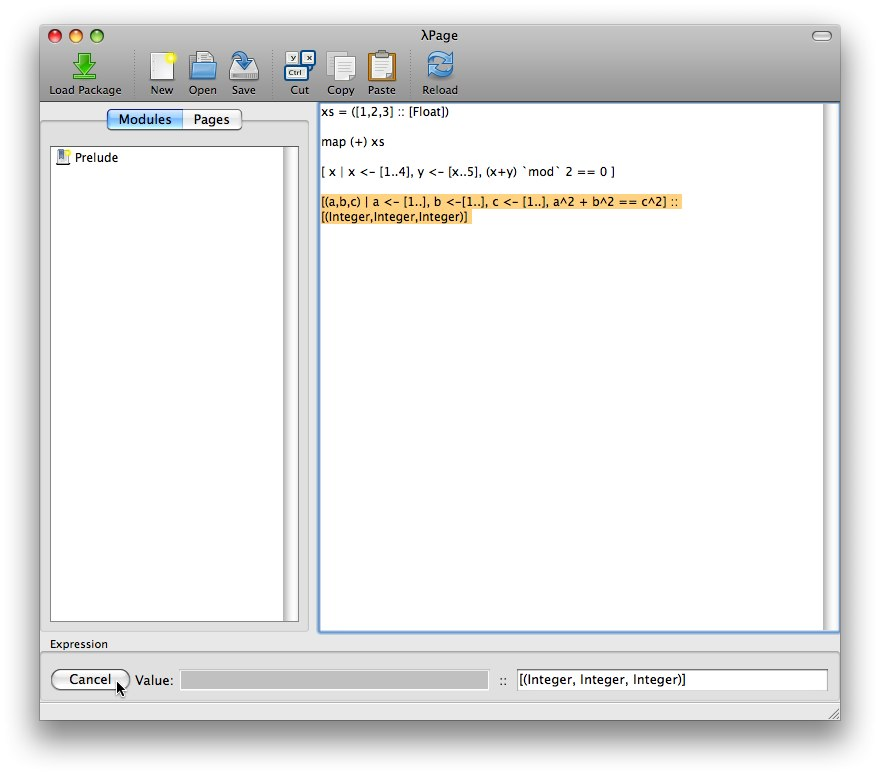
\includegraphics[width=.75\textwidth]{pictures/tut1/03}
		\caption{Tutorial 1 - Ejercicio 5 - Primer intento}
		\label{tut103}
	\end{center}
\end{figure}
\subparagraph{}El alumno podr'a observar entonces que el resultado de la interpretaci'on (si bien tiene un tipo v'alido) nunca aparece por pantalla.  Esto se debe al modo en el que se eval'uan las listas por comprensi'on en \haskell: En este caso teniendo tres generadores (\texttt{a}, \texttt{b} y \texttt{c}), para generar el primer elemento de la lista, \haskell\ toma el primer valor posible para \texttt{a} (o sea $1$), el primer valor posible para \texttt{b} (o sea $2$) y luego itera sobre \texttt{c}, con lo que intentar'a verificar en cada paso de esta iteraci'on que $1^{2} + 1^{2} = c$.  Pero $1^{2}+1^{2} = 2$ y sabemos que no existe ning'un n'umero natural que elevado al cuadrado sea $2$, por lo tanto, \haskell\ nunca encontrar'a el primer elemento de esta lista.  \hpage\ permite al alumno, pues, presionar el bot'on \textsl{Cancel} de modo de interrumpir la evaluaci'on y poder continuar trabajando.
\subparagraph{}Luego de presionar el bot'on \textsl{Cancel}, o incluso durante el lapso en el que \hpage\ trata de evaluar la expresi'on, el alumno puede modificar la expresi'on para cumplir con la consigna del ejercicio.  Podr'ia, por ejemplo, reformularla como muestra la figura \ref{tut104} e intentar interpretarla, considerando que, dentro de los n'umeros naturales se cumple que $a > c \Rightarrow a^{2} > c^{2}$ y $b > c \Rightarrow b^{2} > c^{2}$.  \hpage\ entonces, comenzar'a a exhibir resultados hasta que el alumno presione el bot'on \textsl{Cancel}.
\begin{figure}[hp]
	\begin{center}
        	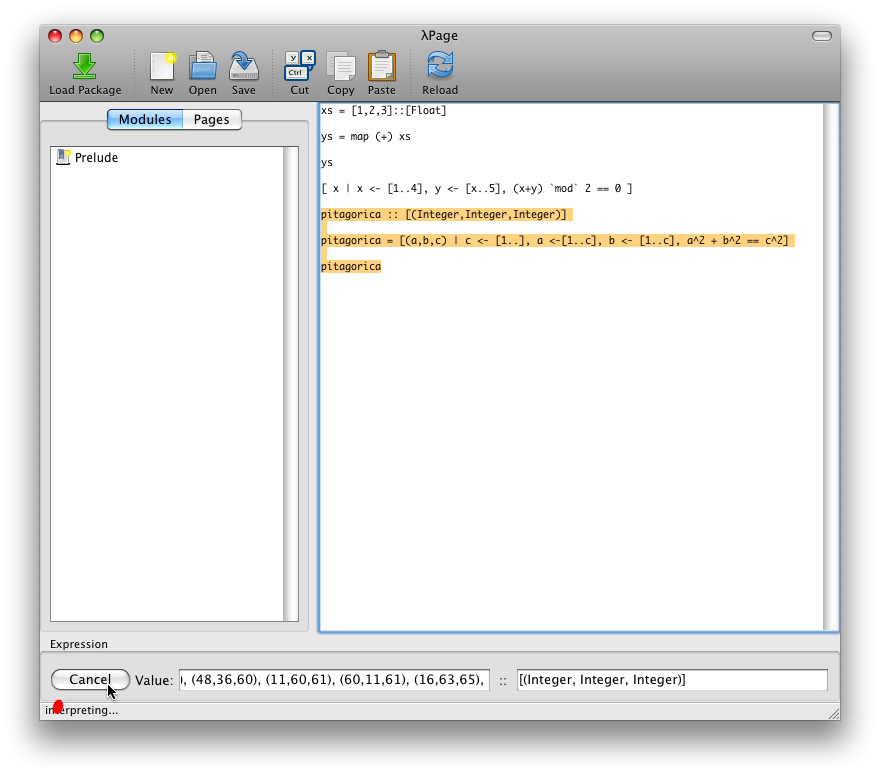
\includegraphics[width=.75\textwidth]{pictures/tut1/04}
		\caption{Tutorial 1 - Ejercicio 5 - Segundo intento}
		\label{tut104}
	\end{center}
\end{figure}
\subparagraph{}Finalmente, el alumno podr'ia tambi'en verificar que puede obtener s'olo las 5 primeras tuplas pitag'oricas, definiendo la serie pitag'orica y tomando s'olo sus primeros 5 elementos como lo muestra la figura \ref{tut105}.  De este modo no necesitar'ia presionar el bot'on \textsl{Cancel}.
\begin{figure}[hp]
	\begin{center}
        	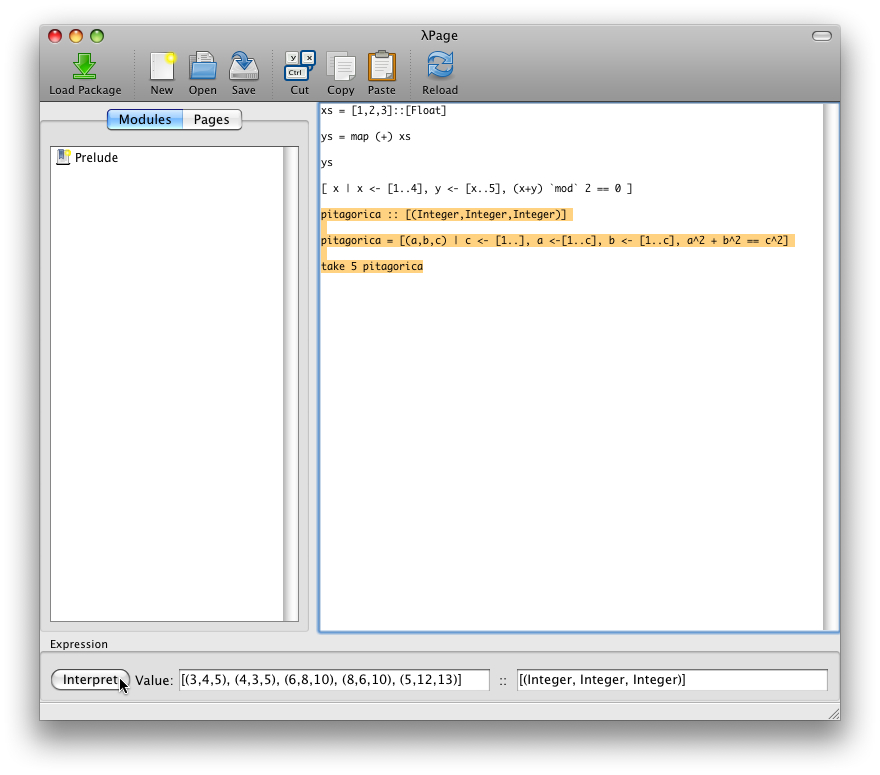
\includegraphics[width=.75\textwidth]{pictures/tut1/05}
		\caption{Tutorial 1 - Ejercicio 5 - Tercer intento}
		\label{tut105}
	\end{center}
\end{figure}

\newpage
\subsubsection{Alto Orden y Esquemas de Recursi'on}
\paragraph{Ejercicio 9}
\renewcommand{\theenumi}{\Roman{enumi}}
\begin{enumerate}
	\item Definir la funci'on \texttt{genLista}, que genera una lista de una cantidad dada de elementos, a partir de un elemento inicial y de una funci'on de incremento entre los elementos de la lista.  Dicha funci'on de incremento, dado un elemento de la lista, devuelve el elemento siguiente.
	\item Usando \texttt{genLista}, definir la funci'on \texttt{dh}, que dado un par de n'umeros (el primero menor que el segundo), devuelve una lista de n'umeros consecutivos desde el primero hasta el segundo.
\end{enumerate}
\renewcommand{\theenumi}{\arabic{enumi}}
\subparagraph{Resoluci'on}En este caso, ciertamente \hpage\ no puede ayudar al alumno a \textsl{crear} las funciones que se le solicitan, pero s'i puede ayudarlo a testearlas.  Supongamos pues que el alumno crea una nueva p'agina y define en ella las funciones \texttt{genLista} y \texttt{dh} tal como se ve en la figura \ref{tut106}.  Luego, intenta testear su ejercicio y, tal como se ve en la figura \ref{tut107}, puede comprobar que sus funciones generan una recursi'on infinita.  Observa entonces que a \texttt{genLista} le falta un \textbf{caso base} y lo agrega, para luego volver a testear sus funciones como se ve en la figura \ref{tut108} y obtener as'i el resultado esperado.
\begin{figure}[hp]
	\begin{center}
        	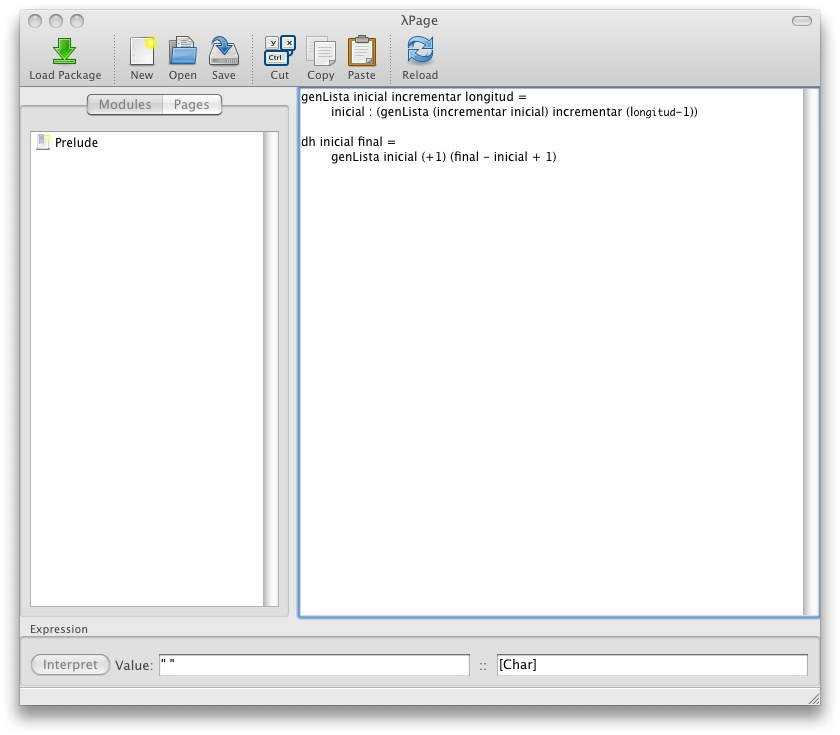
\includegraphics[width=.75\textwidth]{pictures/tut1/06}
		\caption{Tutorial 1 - Ejercicio 9 - Primer Intento}
		\label{tut106}
	\end{center}
\end{figure}
\begin{figure}[hp]
	\begin{center}
        	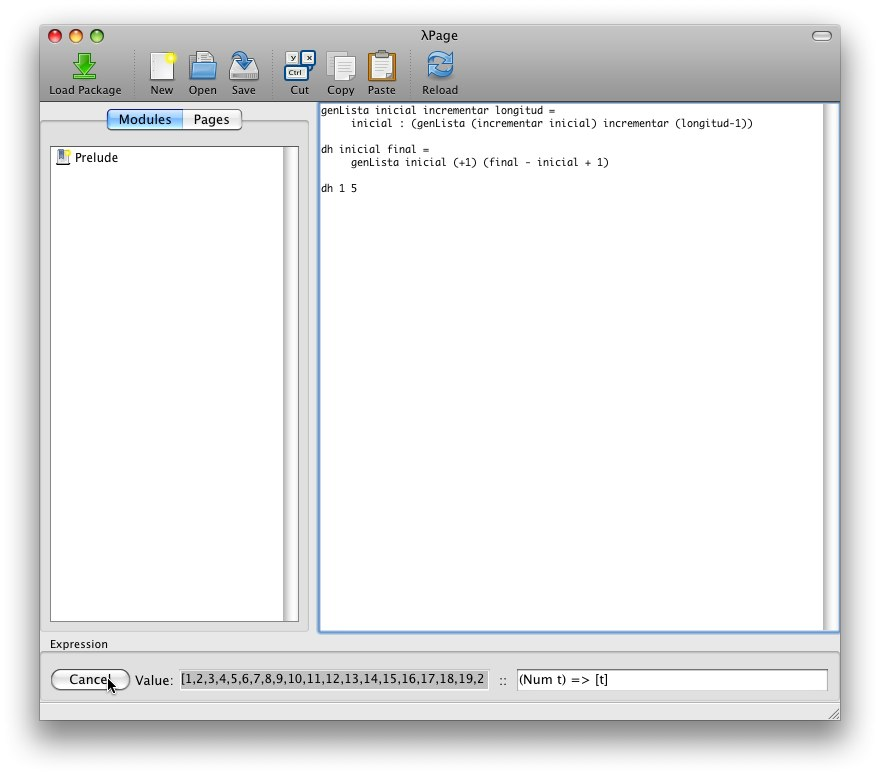
\includegraphics[width=.75\textwidth]{pictures/tut1/07}
		\caption{Tutorial 1 - Ejercicio 9 - Recursi'on Infinita}
		\label{tut107}
	\end{center}
\end{figure}
\begin{figure}[hp]
	\begin{center}
        	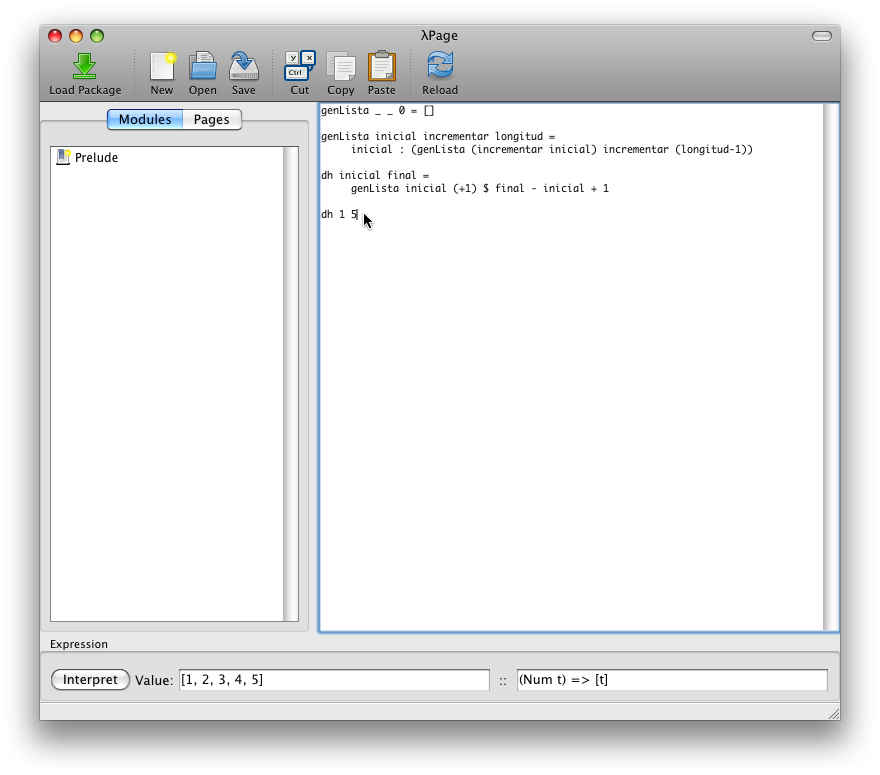
\includegraphics[width=.75\textwidth]{pictures/tut1/08}
		\caption{Tutorial 1 - Ejercicio 9 - Segundo Intento}
		\label{tut108}
	\end{center}
\end{figure}
\subparagraph{}Cabe aclarar que lo hecho en este ejercicio no es (ni pretende tampoco) ser un completo test de las funciones creadas.  Es simplemente lo que hemos llamado \textsl{micro-testing}: El ejercicio de realizar peque'nas pruebas ``a mano'' utilizando expresiones cuyo resultado de evaluaci'on es previsible.

\newpage
\paragraph{Ejercicio 23}Definimos el siguiente tipo:
\begin{center}\begin{lstlisting}
	data Agenda p t = Vacia | Telefonos p [t] (Agenda p t)
\end{lstlisting}\end{center}
\subparagraph{}Este tipo modela una agenda de tel'efonos.  A una agenda se le puede agregar una nueva entrada, donde se registra para una persona una lista de tel'efonos.  Una misma persona puede aparecer en varias entradas.  La lista de tel'efonos de una entrada puede contener repetidos.  Ejemplo:
\begin{center}\begin{lstlisting}
miAgenda = Telefonos "Letincho" [42079999,43834567] 
           (Telefonos "Javi" [47779830] (Telefonos "Letincho" [42079999] Vacia)) 
\end{lstlisting}\end{center}
\ldots
\subparagraph{Resoluci'on}El ejercicio contin'ua, pero en este caso, el alumno podr'ia verse tentado a intentar evaluar \texttt{miAgenda} directamente en \hpage\ y obtendr'ia el resultado de la figura \ref{tut109}.  'Esto se debe a que \hpage\ no soporta definiciones de tipos de datos directamente en el texto.
\begin{figure}[hp]
	\begin{center}
        	
\includegraphics[width=.75\textwidth]{pictures/tut1/09}
		\caption{Tutorial 1 - Ejercicio 23 - Primer Intento}
		\label{tut109}
	\end{center}
\end{figure}
\subparagraph{}Para conseguir el efecto deseado, el alumno puede crear un m'odulo (sin salir de \hpage) y guardarlo utilizando la opci'on \textsl{Page $\rightarrow$ Save As\ldots} o el bot'on \textsl{Save}) tal como se observa en la figura \ref{tut110}.  Luego, utilizando la opci'on \textsl{Haskell $\rightarrow$ Load Modules\ldots} puede cargar el m'odulo reci'en creado, seleccionar la expresi'on \texttt{miAgenda} y evaluarla normalmente.  Observamos el resultado de esta operaci'on en la figura \ref{tut111}
\begin{figure}[hp]
	\begin{center}
        	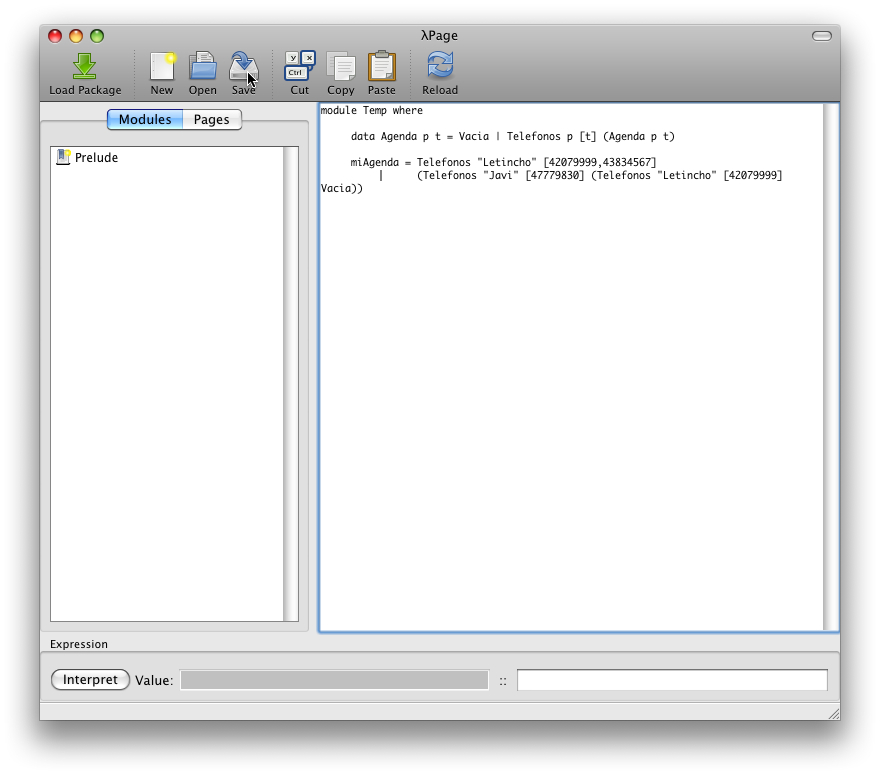
\includegraphics[width=.75\textwidth]{pictures/tut1/10}
		\caption{Tutorial 1 - Ejercicio 23 - Crear M'odulo}
		\label{tut110}
	\end{center}
\end{figure}
\begin{figure}[hp]
	\begin{center}
        	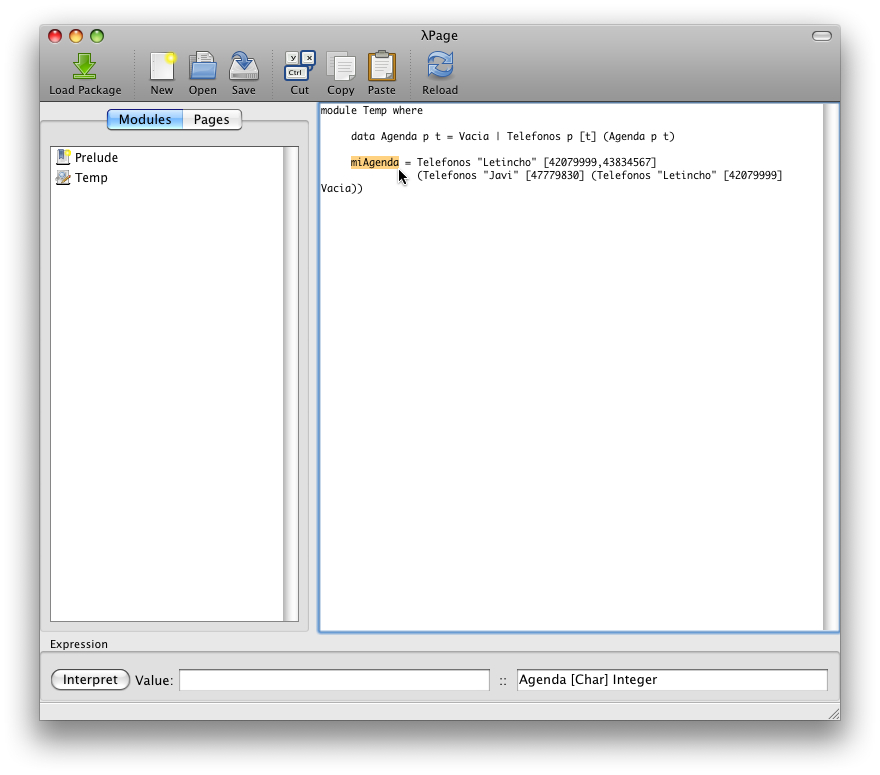
\includegraphics[width=.75\textwidth]{pictures/tut1/11}
		\caption{Tutorial 1 - Ejercicio 23 - Segundo Intento}
		\label{tut111}
	\end{center}
\end{figure}
\subparagraph{}Podemos ver, por un lado, que el resultado no ha sido mostrado, sino que s'olo se inform'o su tipo.  Esto se debe a que el tipo \texttt{Agenda} no es instancia de la clase \texttt{Show}.  Para visualizar el resultado, el alumno podr'ia agregar la cl'ausla \texttt{deriving (Show)} al tipo \texttt{Agenda}, grabar el m'odulo modificado, presionar el bot'on \textsl{Reload} y luego evaluar nuevamente \texttt{miAgenda} tal como se ve en la figura \ref{tut112}.
\begin{figure}[hp]
	\begin{center}
        	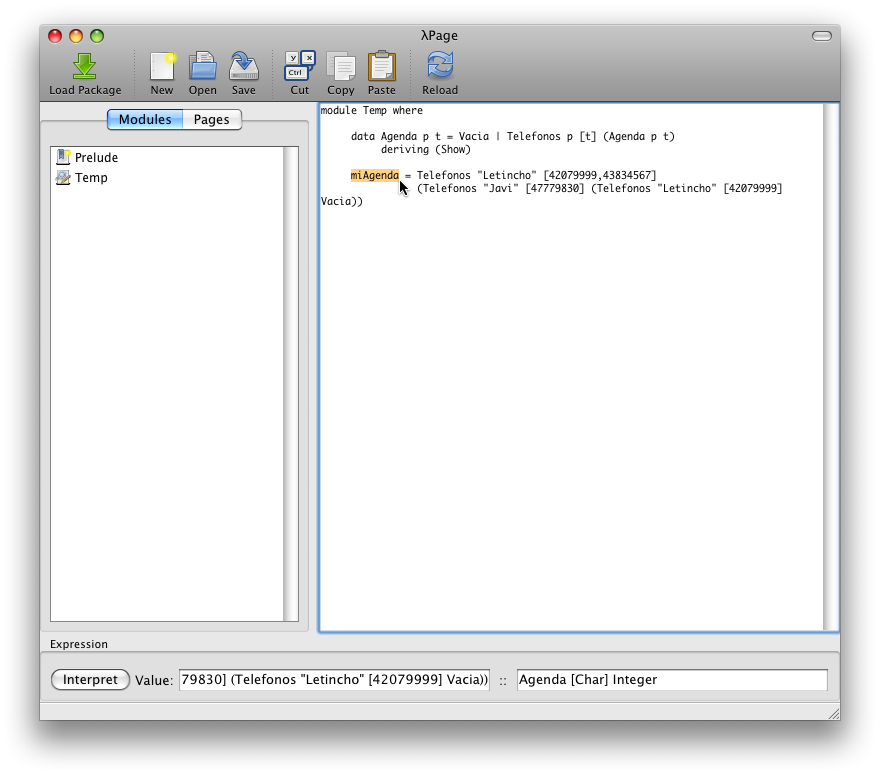
\includegraphics[width=.75\textwidth]{pictures/tut1/12}
		\caption{Tutorial 1 - Ejercicio 23 - Tercer Intento}
		\label{tut112}
	\end{center}
\end{figure}
\subparagraph{}Por otra parte, aprovecharemos este ejercicio simple para mostrar lo que \hpage\ permite hacer con los elementos de la lista \textsl{Modules}.  Presionando bot'on derecho del mouse sobre un 'item, \hpage\ despliega un men'u que nos permite, entre otras opciones ``navegar''  el m'odulo y observar los elementos que exporta.  La figura \ref{tut113} nos muestra el ``'arbol'' que se desprende de nuestro m'odulo \texttt{Temp}
\begin{figure}[hp]
	\begin{center}
        	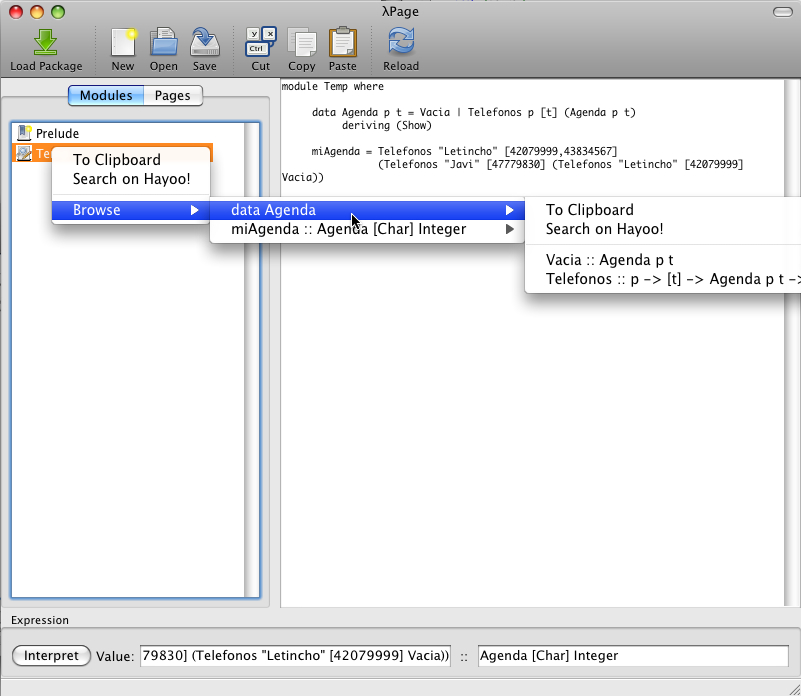
\includegraphics[width=.75\textwidth]{pictures/tut1/13}
		\caption{Tutorial 1 - Navegando M'odulos}
		\label{tut113}
	\end{center}
\end{figure}

\newpage
\subsubsection{Conclusiones}
\paragraph{}En este tutorial hemos demostrado un uso sencillo de \hpage\ como herramienta de \textsl{micro-testing}, permitiendo al usuario trabajar con las funciones definidas en el \texttt{Prelude} de \haskell\ adem'as de las que 'el mismo desee definir localmente.
\paragraph{}Pudimos apreciar c'omo \hpage\ permite definir expresiones y funciones, para luego evaluarlas de manera individual o combinada.  Dichas evaluaciones pueden generar diversos resultados y hemos visto c'omo se maneja \hpage\ con algunos de ellos:
\begin{itemize}
\item Para aquellas expresiones cuyo valor no puede ser expresado en forma de texto, hemos visto c'omo \hpage\ nos permite conocer su tipo.
\item En el caso de expresiones cuyo valor es de longitud infinita, \hpage\ exhibe todo lo que el usuario desee del resultado, culminando cuando 'este presiona el bot'on \textsl{Cancel}.
\item Y en relaci'on a aquellas que requieren un c'alculo infinito para determinar su valor, \hpage\ muestra su tipo y permite al usuario continuar trabajando con las dem'as expresiones hasta que decida presionar el bot'on \textsl{Cancel} e interrumpir de esa manera el c'alculo.
\end{itemize}
\paragraph{}Esta forma de trabajar con los resultados, combinada con la posibilidad que brinda \hpage\ de editar definiciones de manera simple y directa, para luego volver a evaluar expresiones que las usan, permite al usuario trabajar fluidamente y le da la libertad de \textsl{cometer errores}, detectarlos, corregirlos y luego continuar su trabajo.  Esta caracter'istica de \hpage\ es muy importante sobre todo para quienes se encuentran dando sus primeros pasos en el mundo de \haskell\ pues, entendemos, facilita el aprendizaje del lenguaje.
\paragraph{}Tambi'en hemos visto en este tutorial c'omo se puede utilizar \hpage\ para crear, cargar, modificar y recargar m'odulos, trabajando siempre en una 'unica p'agina de texto.  'Esta es otra caracter'istica de \hpage\ que facilita el trabajo ya no s'olamente a los estudiantes sino a todo tipo de desarrolladores \haskell.

\newpage
\subsection{Caso de Uso: Ganando al 4 en L'inea con \hpage}
\begin{epigraphs}
	\qitem{We learn by example and by direct experience because there are real limits to the adequacy of verbal instruction}{Malcom Gladwell}
	\qitem{Look behind you, a Three-Headed Monkey!}{Guybrush Threepwood}
\end{epigraphs}
\paragraph{}Inclu'imos en este informe un segundo tutorial, apuntando esta vez a demostrar c'omo \hpage\ puede ser de utilidad para un programador \haskell\ que se enfrenta a un problema m'as lejano al mundo acad'emico.  En 'el veremos c'omo trabajar con herramientas tales como \cabal, \textsl{Hayoo!} y \textsl{wxHaskell}.  Veremos como \hpage\ ayuda al usuario a ``entender'' c'odigo escrito por otra persona (o quiz'a por el mismo, alg'un tiempo atr'as).
\subsubsection{Introducci'on}
\paragraph{}La historia comienza cuando nuestra amiga desarrolladora, a quien llamaremos \textsl{F'atima}\footnote{El nombre lo hemos elegido en honor a quien, hace ya casi 15 a'nos y utilizando el sobrenombre \textsl{Pers'efone}, fue la \textsl{maestra} y principal rival de 4 en L'inea de Fernando Benavides en \htmladdnormallink{CyberJuegos}{http://www.cyberjuegos.com}} para darle un poco de personalidad, se encuentra con la misi'on de modificar una implementaci'on de un juego de \textsl{4 en L'inea}, llamada \htmladdnormallink{hfiar}{http://hackage.haskell.org/package/hfiar}~\cite{hfiar}.  F'atima tiene que adaptar el juego de modo que permita \textsl{jugar contra la computadora} pues actualmente s'olo permite jugar a dos seres humanos entre s'i.
\subparagraph{}Como es de suponer, F'atima no conoce al creador del juego y no puede contactarlo por lo que sus 'unicas herramientas, m'as all'a de su conocimiento de \haskell\ y del juego en s'i, son el c'odigo fuente de \textsl{hfiar} y \hpage.

\subsubsection{Primeros Pasos}
\paragraph{}Para comenzar, F'atima descarga el c'odigo del programa desde \textsl{HackageDB} y lo descomprime o bien clona el repositorio \textsl{Git} con el siguiente comando:
\lstset{language=sh, frame=single, tabsize=2}
\begin{center}\begin{lstlisting}
$ git clone git://github.com/elbrujohalcon/hfiar.git
\end{lstlisting}\end{center}
\begin{figure}[hp]
	\begin{center}
        	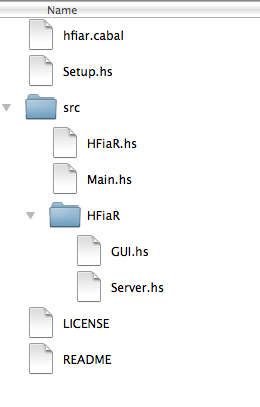
\includegraphics{pictures/tut2/00}
		\caption{Tutorial 2 - Archivos Originales}
		\label{tut200}
	\end{center}
\end{figure}
\paragraph{}Una vez hecho eso, puede observar la estructura del proyecto, tal como se ve en la figura \ref{tut200}.  Conociendo la estructura b'asica de los proyectos desarrollados en \haskell, podemos describir los archivos all'i presentes de la siguiente manera:
\begin{description}
\item[hfiar.cabal] Archivo de descripci'on de proyecto \cabal.  F'atima puede obtener de 'el informaci'on general del proyecto, sus m'odulos, las extensiones que se necesitan para compilarlo y dem'as.  
\item[Setup.hs] Archivo \haskell\ utilizado por \cabal\ para realizar tareas especiales al momento de configurar, compilar o instalar la aplicaci'on.  Junto con \textbf{hfiar.cabal} permite instalar el proyecto utilizando las instrucciones de la figura \ref{tut201}.
\begin{figure}[hp]
	\begin{center}
		\begin{center}\begin{lstlisting}
$ cabal configure --user
$ cabal build
$ cabal install
		\end{lstlisting}\end{center}
		\caption{Tutorial 2 - Instalaci'on}
		\label{tut201}
	\end{center}
\end{figure}
\item[src] Carpeta que contiene los archivos de c'odigo fuente del proyecto.  F'atima deber'a analizar cada uno de ellos por separado para poder comprender su funcionamiento.
\item[LICENSE] Tradicional archivo con la descripci'on de la licencia del proyecto.
\item[README] En el caso de este proyecto, no se trata de algo demasiado 'util, dice simplemente:
\begin{verbatim}
Four in a Row in Haskell!!
See http://hackage.haskell.org/package/hfiar
\end{verbatim}
\end{description}

\newpage
\subsubsection{Entendiendo el Proyecto}
\paragraph{}Para comenzar a entender c'omo est'a estructurada la aplicaci'on, F'atima observa el archivo \textbf{hfiar.cabal} (al que podemos ver en la figura \ref{tut202}) y observa que el proyecto se encuentra compuesto por una librer'ia (que incluye s'olamente al m'odulo \texttt{HFiaR}) y un ejecutable llamado \texttt{hfiar} que, m'as all'a del m'odulo \texttt{Main}, incluye a los m'odulos \texttt{HFiaR.GUI} y \texttt{HFiaR.Server}.  F'atima puede ver adem'as que, para compilar los m'odulos del proyecto, debe utilizar las extensiones \textbf{MultiParamTypeClasses} y \textbf{GeneralizedNewtypeDeriving}.
\begin{figure}[hp]
	\begin{center}
	\hbox{}
		\begin{center}\begin{lstlisting}
name: hfiar
version: 1.0.0
cabal-version: >=1.6
build-type: Custom
license: BSD3
license-file: LICENSE
copyright: 2010 Fernando "Brujo" Benavides
maintainer: greenmellon@gmail.com
stability: stable
homepage: http://github.com/elbrujohalcon/hfiar
package-url: http://code.haskell.org/hfiar
bug-reports: http://github.com/elbrujohalcon/hfiar/issues
synopsis: Four in a Row in Haskell!!
description: The classical game, implemented with wxHaskell
category: Game
author: Fernando "Brujo" Benavides
tested-with: GHC ==6.10.4
data-files: LICENSE README
data-dir: ""
extra-source-files: Setup.hs
extra-tmp-files:

source-repository head
    type:     git
    location: git://github.com/elbrujohalcon/hfiar.git

Library
    build-depends: base >= 4,                   base < 5,
                   mtl >=1.1.0,                 mtl < 1.2,
                   eprocess >= 1.1.0,           eprocess < 2
    extensions: MultiParamTypeClasses, GeneralizedNewtypeDeriving
    exposed-modules: HFiaR
    hs-source-dirs: src

Executable hfiar
    build-depends: wxcore >=0.11.1,             wxcore < 0.13,
                   wx >=0.11.1,                 wx < 0.13
    extensions: MultiParamTypeClasses, GeneralizedNewtypeDeriving
    main-is: Main.hs
    buildable: True
    hs-source-dirs: src
    other-modules: HFiaR.GUI, HFiaR.Server
    ghc-options: -fwarn-unused-imports -fwarn-missing-fields
                 -fwarn-incomplete-patterns
		\end{lstlisting}\end{center}
		\caption{Tutorial 2 - hfiar.cabal}
		\label{tut201}
	\end{center}
\end{figure}
\subparagraph{}Habiendo realizado este an'alisis, F'atima configura el proyecto ejecutando la siguiente instrucci'on:
\begin{center}\begin{lstlisting}
$ cabal configure --user
\end{lstlisting}\end{center}
\subparagraph{}Sabiendo que existe una librer'ia en el proyecto, F'atima intenta generar su documentaci'on, ejecutando:
\begin{center}\begin{lstlisting}
$ cabal haddock
\end{lstlisting}\end{center}
\subparagraph{}En el caso de \textsl{hfiar}, ese comando genera la documentaci'on en formato HTML, siendo su p'agina principal \texttt{dist/doc/html/hfiar/index.html}.  F'atima encuentra all'i una descripci'on de los componentes del m'odulo \texttt{HFiaR}.  Armada con estos datos, se dispone a utilizar \hpage\ para comprender c'omo funcionan esos componentes.

\newpage
\subsubsection{Utilizando \hpage}
\paragraph{}Una vez abierto \hpage, F'atima intentar cargar el proyecto utilizando la opci'on \textsl{Haskell $\rightarrow$ Load Package\ldots} o el bot'on \textsl{Load Package}.  Eso abre una ventana en la que F'atima debe seleccionar el archivo \textbf{setup-config} generado por \cabal, tal como se ve en la figura \ref{tut202}.
\begin{figure}[hp]
	\begin{center}
        	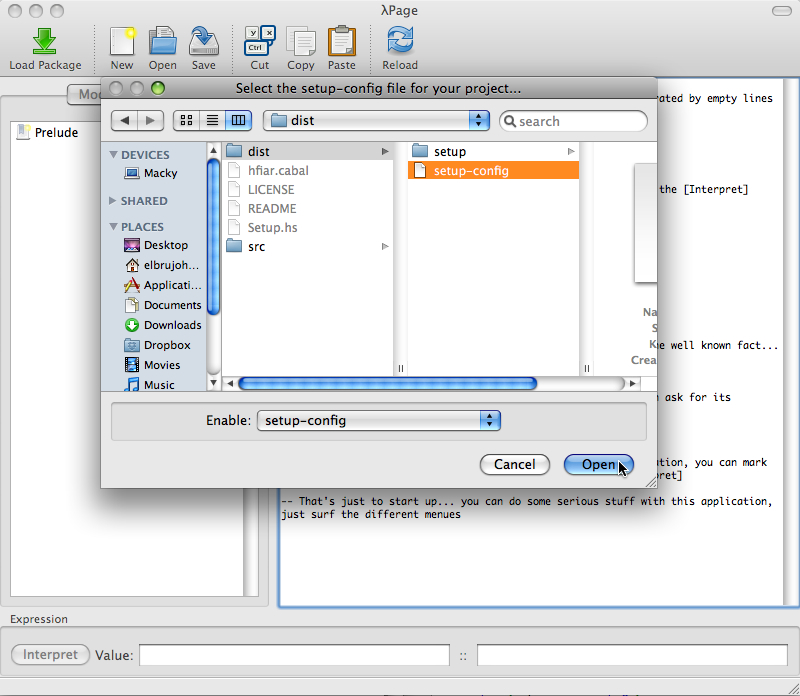
\includegraphics[width=.75\textwidth]{pictures/tut2/02}
		\caption{Tutorial 2 - Cargando un proyecto \cabal}
		\label{tut202}
	\end{center}
\end{figure}
\subparagraph{}F'atima tendr'a entonces a su disposici'on los m'odulos que componen la aplicaci'on y, haciendo click derecho en ellos, podr'a cargarlos, como se ve en la figura \ref{tut203}.
\begin{figure}[hp]
	\begin{center}
        	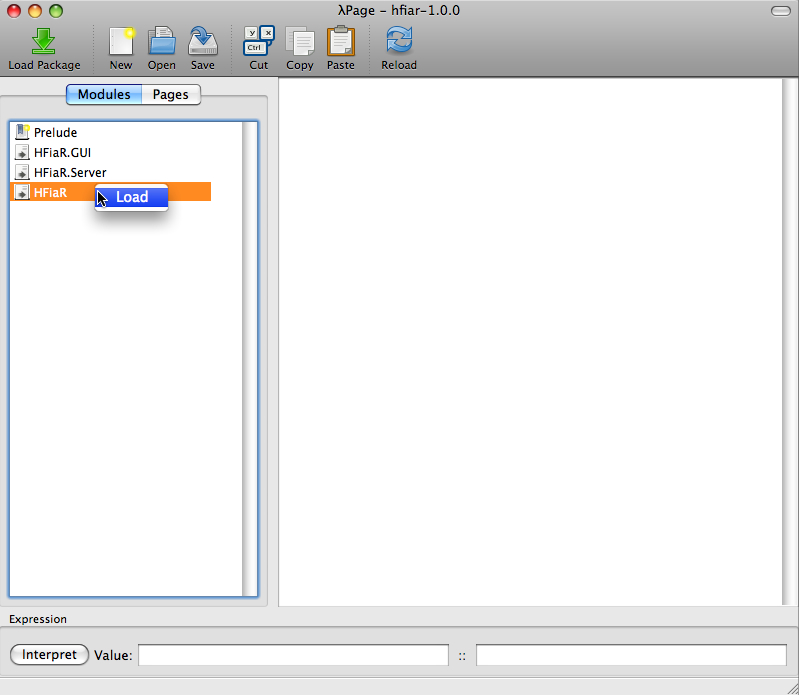
\includegraphics[width=.75\textwidth]{pictures/tut2/03}
		\caption{Tutorial 2 - Proyecto \cabal\ cargado}
		\label{tut203}
	\end{center}
\end{figure}
\newpage
\paragraph{}Recordando que el proyecto inclu'ia una librer'ia compuesta 'unicamente por el m'odulo \texttt{HFiaR}, nuestra amiga F'atima decide cargarlo y navegarlo utilizando el men'u desplegable que nos muestra la figura \ref{tut204}.
\begin{figure}[hp]
	\begin{center}
        	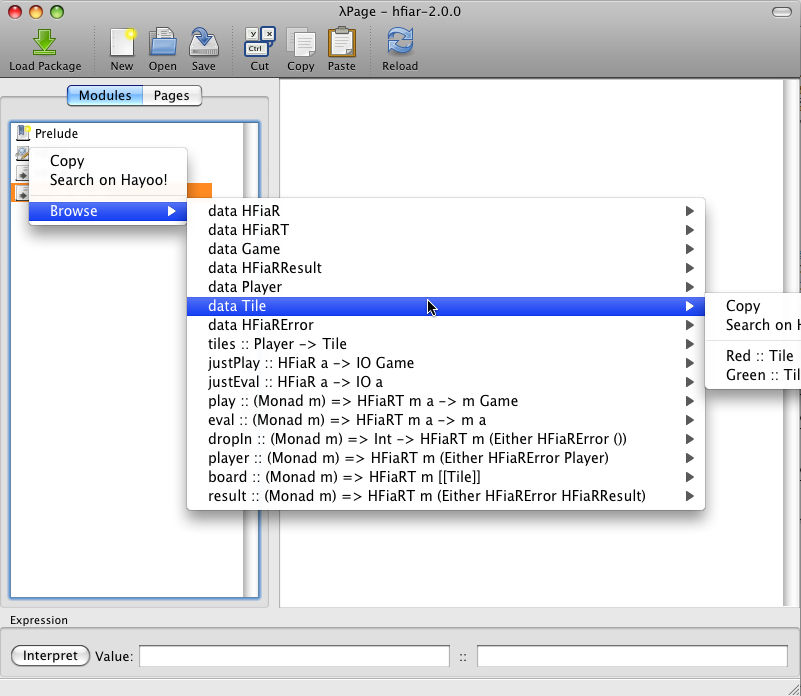
\includegraphics[width=.75\textwidth]{pictures/tut2/04}
		\caption{Tutorial 2 - M'odulo \texttt{HFiaR}}
		\label{tut204}
	\end{center}
\end{figure}
\paragraph{}Gracias a la documentaci'on generada previamente, puede observar que la din'amica del juego est'a modelada con una m'onada que permite describir las acciones llevadas a cabo durante un partido (b'asicamente utilizando la funci'on \texttt{dropIn}, que equivale a la acci'on que realiza el jugador actual al momento de dejar caer una ficha en una columna).  Esta m'onada tambi'en permite observar un juego utilizando las funciones \texttt{player} (para conocer el jugador actual), \texttt{board} (para observar el tablero, que es modelado como una lista de listas de \texttt{Tile}s, o sea fichas) y \texttt{result} para verificar el resultado del partido.
\subparagraph{}Puede ver tambi'en que dichas acciones pueden ser ejecutadas dentro de cualquier m'onada, gracias a las funciones \texttt{play} y \texttt{eval} y al hecho de que la m'onada est'a implementada utilizando la t'ecnica de \textsl{Monad Transformers}~\cite{realworldhaskell}.
\subparagraph{}Finalmente, y de modo muy conveniente, F'atima observa que el creador del m'odulo provey'o las funciones \texttt{justPlay} y \texttt{justEval} que permiten simplemente ejecutar las acciones de la m'onada y obtener su resultado.  Utilizando estas funciones, F'atima comienza a realizar su tarea de \textsl{micro-testing}.  Su primera prueba consiste en \textit{jugar} un partido en el que nada pasa, s'olo para ver qu'e informaci'on puede obtener de 'el.  Coloca entonces en la p'agina la expresi'on que presentamos a continuaci'on e intenta interpretarla tal como se ve en la figura \ref{tut205}
\lstset{language=haskell, frame=single, tabsize=4}
\begin{center}\begin{lstlisting}
	justPlay $ return ()
\end{lstlisting}\end{center}
\begin{figure}[hp]
	\begin{center}
        	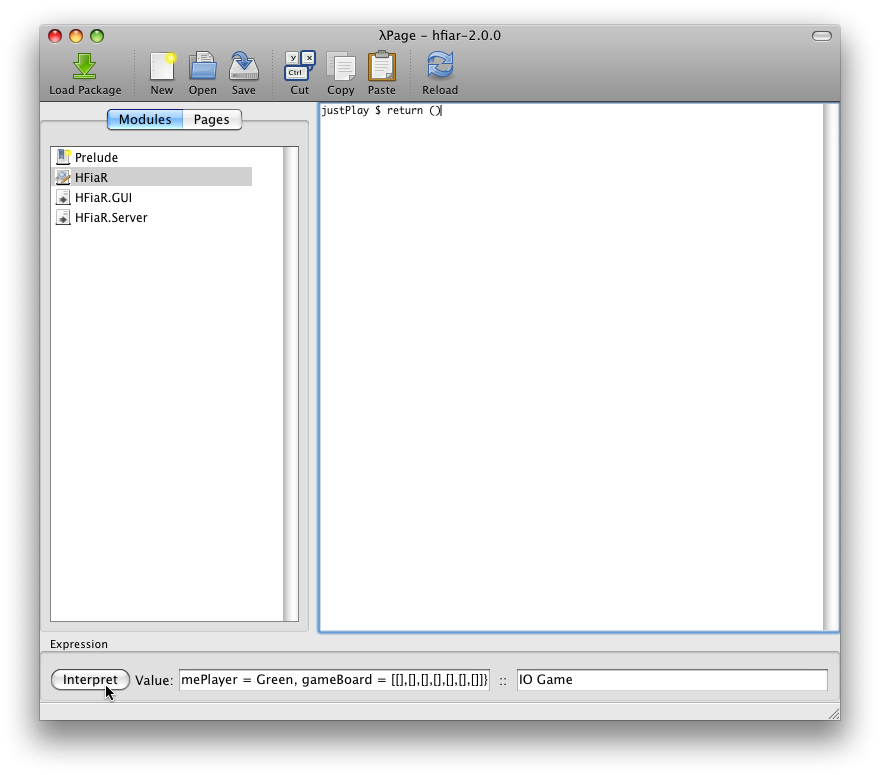
\includegraphics[width=.75\textwidth]{pictures/tut2/05}
		\caption{Tutorial 2 - Juego M'inimo}
		\label{tut205}
	\end{center}
\end{figure}
\subparagraph{}El resultado obtenido es el que sigue y puede interpretarse como \textsl{``el partido se encuentra en curso, es el turno del jugador que juega con fichas verdes y el tablero est'a vac'io''}.
\begin{center}\begin{lstlisting}
OnCourse {gamePlayer = Green,
          gameBoard = [[],[],[],[],[],[],[]]}
\end{lstlisting}\end{center}
\newpage
\paragraph{}Usando \hpage, F'atima realiza varias otras pruebas que consignamos en la tabla del cuadro \ref{tut206}.  Con ellas puede entender el funcionamiento general de la m'onada \texttt{HFiaR} y de ese modo determinar c'omo su jugador de inteligencia artificial puede observar el desarrollo del juego (saber si el mismo ha concluido o no, si es su turno y el estado del tablero) y elegir c'omo jugar.  Cabe notar que los resultados de tipo \texttt{Left HFiaRError} se exhiben como texto porque el desarrollador de \textsl{hfiar} ha decidido utilizar la funci'on \texttt{show} para describir los errores en lugar de exhibir su constructor.

\lstset{language=haskell, frame=none, tabsize=4}
	\begin{table}[hp]
		\begin{center}
			\begin{tabular}{@{} cc @{}}
				\toprule
				Expresi'on & Resultado \\ 
				\midrule
\begin{lstlisting}
justPlay $ return ()
\end{lstlisting} &
\begin{lstlisting}
OnCourse {gamePlayer = Green,
          gameBoard = [[],[],[],[],[],[],[]]}
\end{lstlisting} \\[1.5em]

\begin{lstlisting}
justEval $ player
\end{lstlisting} &
\begin{lstlisting}
Right Green
\end{lstlisting} \\[1.5em]

\begin{lstlisting}
justEval $ dropIn 1 >> board
\end{lstlisting} &
\begin{lstlisting}
[[],[Green],[],[],[],[],[]]
\end{lstlisting} \\[1.5em]

\begin{lstlisting}
justEval $ dropIn 7
\end{lstlisting} &
\begin{lstlisting}
Left That column doesn't exist
\end{lstlisting} \\[1.5em]

\begin{lstlisting}
justPlay $ dropIn 4 >> dropIn 1 >>
           dropIn 4 >> dropIn 1 >>
           dropIn 4 >> dropIn 1 >>
           dropIn 4
\end{lstlisting} &
\begin{lstlisting}
Ended {gameResult = WonBy Green,
       gameBoard = [[],[Red,Red,Red],
                    [],[],
                    [Green,Green,Green,Green],
                    [],[]]}
\end{lstlisting} \\[1.5em]

\begin{lstlisting}
justEval $ dropIn 4 >> dropIn 1 >>
           dropIn 4 >> dropIn 1 >>
           dropIn 4 >> dropIn 1 >>
           dropIn 4 >> result
\end{lstlisting} &
\begin{lstlisting}
Right (WonBy Green)
\end{lstlisting} \\[1.5em]

\begin{lstlisting}
justEval $ dropIn 4 >> dropIn 1 >>
           dropIn 4 >> dropIn 1 >>
           dropIn 3 >> dropIn 1 >>
           dropIn 4 >> result
\end{lstlisting} &
\begin{lstlisting}
Left Game is on course yet
\end{lstlisting} \\[1.5em]

\begin{lstlisting}
justEval $ dropIn 1 >> dropIn 1 >>
           dropIn 1 >> dropIn 1 >>
           dropIn 1 >> dropIn 1 >>
           dropIn 1 >> dropIn 1
\end{lstlisting} &
\begin{lstlisting}
Left That column is full
\end{lstlisting} \\[1.5em]

			\bottomrule
		\end{tabular}
		\caption{Tutorial 2 - Pruebas realizadas en \hpage}
		\label{tut206}
	\end{center}
\end{table}
\lstset{language=haskell, frame=single, tabsize=4}

\newpage
\subsubsection{Creando al \textsl{Jugador Computadora}}
\paragraph{}Con el conocimiento adquirido en el uso de \texttt{HFiaR}, F'atima decide crear la funci'on \texttt{aiDropIn}, que se ejecutar'a dentro de la m'onada \texttt{HFiaR}.  La figura \ref{tut207} nos muestra la aridad de dicha funci'on.
\begin{figure}[hp]
	\begin{center}
		\begin{lstlisting}
-- | Drop a tile in a column choosen by the Artificial Inteligence
aiDropIn :: Monad m => HFiaRT m (Either HFiaRError ())
		\end{lstlisting}
		\caption{Tutorial 2 - Aridad de aiDropIn}
		\label{tut207}
	\end{center}
\end{figure}
\subparagraph{}Para crear \texttt{aiDropIn}, F'atima no cierra \hpage.  Por el contrario, define la funci'on all'i mismo, como podemos ver en la figura \ref{tut208}, componi'endola con otra funci'on a la que denomina \texttt{bestColumnFor}.  Esta funci'on se ejecutar'a fuera del contexto mon'adico y s'olo en el caso de que el partido no haya concluido.  La idea es que en ella estar'a el algoritmo principal de selecci'on de columna a jugar (o sea, el verdadero motor de \textsl{inteligencia artificial}), el cual se ir'a perfeccionando paso a paso.  La primera versi'on de \texttt{bestColumnFor}, con m'as de artificial que de inteligencia, simplemente elegir'a la primer columna que no est'e llena y \texttt{aiDropIn} arrojar'a la ficha ah'i.
\begin{figure}[hp]
	\begin{center}
        	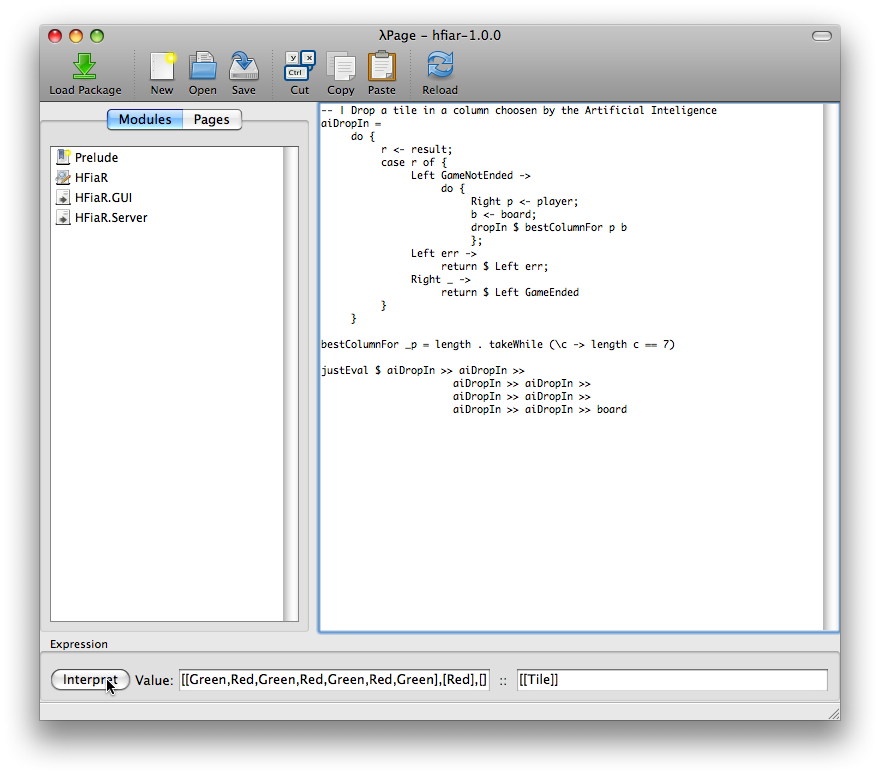
\includegraphics[width=.75\textwidth]{pictures/tut2/06}
		\caption{Tutorial 2 - \texttt{aiDropIn} versi'on 1}
		\label{tut208}
	\end{center}
\end{figure}
\subparagraph{}Una vez definidas ambas funciones, F'atima decide testearlas y, para ello, no necesita m'as que \textsl{evaluar} un juego en el que conozca el resultado.  En particular, F'atima elije hacer jugar a la computadora contra s'i misma 8 movimientos y verifica que las fichas han quedado intercaladas en la primer columna y luego el siguiente jugador ha colocado una en la segunda.
\paragraph{}El siguiente paso es agregar un poco de inteligencia a \texttt{bestColumnFor} de modo que realmente sea competitivo.  Para ello, F'atima prev'e que necesitar'a varias funciones auxiliares y una buena cantidad de c'odigo, por lo que decide convertir su p'agina actual en un m'odulo al que denomina \texttt{HFiaR.AI} y graba en el lugar correspondiente entre los fuentes del proyecto, utilizando la opci'on \textsl{Page $\rightarrow$ Save As\ldots} o el bot'on \textsl{Save} tal como se observa en la figura \ref{tut208}.  Luego lo carga utilizando la opci'on \textsl{Haskell $\rightarrow$ Load Modules\ldots} y, seleccionando \texttt{testGame} puede realizar la misma prueba de la figura \ref{tut207}.  Es interesante notar que, pese a que el m'odulo creado s'olo exporta la funci'on \texttt{aiDropIn}, F'atima pudo interpretar sin problemas la funci'on \texttt{testGame}, pues hab'ia cargado el m'odulo y eso le da acceso a todas las funciones del mismo, tanto p'ublicas como privadas.
\begin{figure}[hp]
	\begin{center}
        	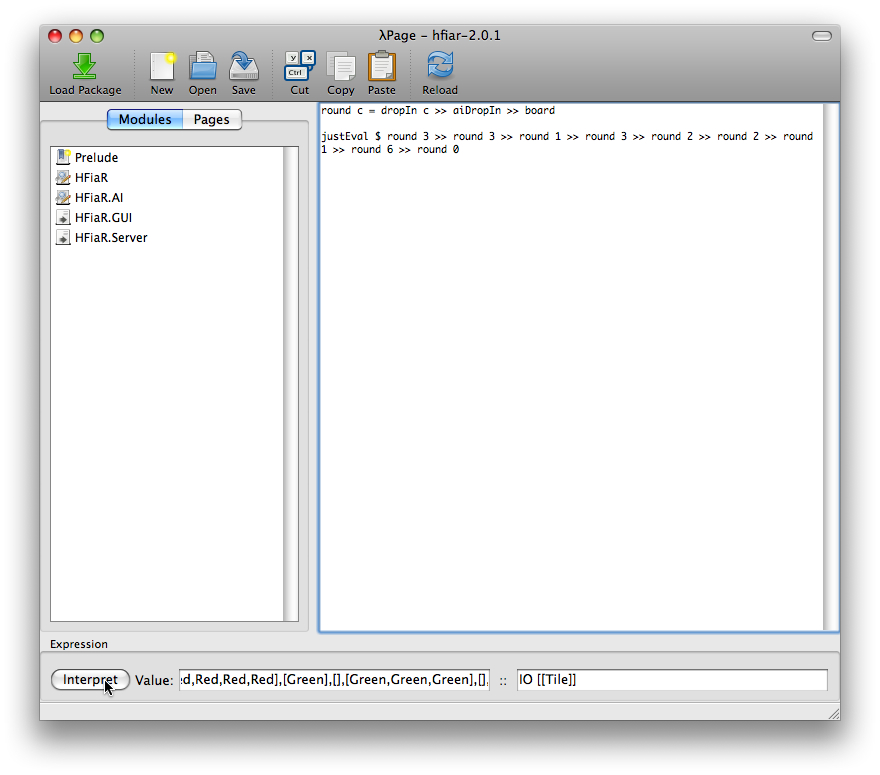
\includegraphics[width=.75\textwidth]{pictures/tut2/08}
		\caption{Tutorial 2 - El m'odulo \texttt{HFiaR.AI}}
		\label{tut208}
	\end{center}
\end{figure}
\newpage
\subparagraph{}Para la segunda (y a los fines de este tutorial, definitva) versi'on de \texttt{bestColumnFor}, F'atima, experta jugadora de 4 en l'inea como es, pone un poco de criterio y decide que la funci'on tenga en cuenta las condiciones que enumeramos a continuaci'on.  La nueva versi'on de \texttt{bestColumnFor} y sus funciones adicionales las podemos observar en la figura \ref{tut209}.  El resto del m'odulo permanece tal como estaba.
\begin{itemize}
	\item Si poniendo la ficha en alguna columna el jugador gana el partido, se debe elegir esa columna.
	\item Si poniendo la ficha en alguna columna se impide que el jugador rival gane el partido (pues acumula 3 alineadas convenientemente) se debe elegir esa columna.
	\item En otro caso, de ser posible, debe elegirse la columna 3 (o sea, la columna central) pues para formar l'ineas de 4 fichas horizontales o diagonales se requiere una ficha en dicha columna
\end{itemize}
\begin{figure}[hp]
	\begin{center}
		\begin{lstlisting}
bestColumnFor :: Player -> [[Tile]] -> Int
bestColumnFor p b =
	case columnWhereWins p b of
		Nothing ->
			case columnWhereLooses p b of
				Nothing ->
					case length (b !! 3) of
						7 -> length $ takeWhile (\c -> length c == 7) b
						_ -> 3
				Just cwl -> cwl
		Just cww -> cww

columnWhereWins :: Player -> [[Tile]] -> Maybe Int
columnWhereWins Pl{tiles=tile} b =
	case (length $ takeWhile (not . wins tile b) [0..6]) of
		7 -> Nothing
		x -> Just x

columnWhereLooses :: Player -> [[Tile]] -> Maybe Int
columnWhereLooses Pl{tiles=tile} b =
	let otherTile = case tile of {Green -> Red; Red -> Green}
	 in case (length $ takeWhile (not . wins otherTile b) [0..6]) of
			7 -> Nothing
			x -> Just x

wins :: Tile -> [[Tile]] -> Int -> Bool
wins t b c =
	let	newBoard = (take c b) ++ ((t : (b !! c)) : drop (c+1) b)
		col = newBoard !! c
		getRow r = map (cell r)
		getDiagUpRight c r xss = map (\i -> cell (i+r-c) (xss !! i)) [0..6]
		getDiagUpLeft c r xss = map (\i -> cell (r+c-i) (xss !! i)) [0..6]
		cell c xs = if (c >= 0 && c < length xs)
					then Just $ (reverse xs) !! c
					else Nothing
		fourIn [] = False
		fourIn (Nothing:xs) = fourIn xs
		fourIn (Just p:xs) = ([Just p,Just p,Just p] == take 3 xs) || fourIn xs
      in	([t,t,t,t] == take 4 col) ||
      	fourIn (getRow (length col - 1) newBoard) ||
		fourIn (getDiagUpRight c (length col - 1) newBoard) ||
		fourIn (getDiagUpLeft  c (length col - 1) newBoard)
		\end{lstlisting}
		\caption{Tutorial 2 - Versi'on definitiva de \texttt{HFiaR.AI}}
		\label{tut209}
	\end{center}
\end{figure}
\paragraph{} La funci'on \texttt{testGame} ya no es suficiente para testear el funcionamiento de \texttt{aiDropin} pero, como el c'odigo est'a en un m'odulo que ha sido cargado dentro de \hpage, lo que F'atima puede hacer es crear una nueva p'agina utilizando la opci'on \textsl{Page $\rightarrow$ New} e ir construyendo paso a paso una expresi'on que represente un partido entre ella y \textsl{el Jugador Computadora}.  Para ello, define la funci'on auxiliar \texttt{round} y, tal como lo vemos en la figura \ref{tut210}, la utiliza una y otra vez para modificar el partido que pretende ``jugar''.  De ese modo puede probar el comportamiento de su m'odulo de inteligencia artificial ante las distintas circunstancias de un partido tan extenso como ella desee.
\begin{figure}[hp]
	\begin{center}
        	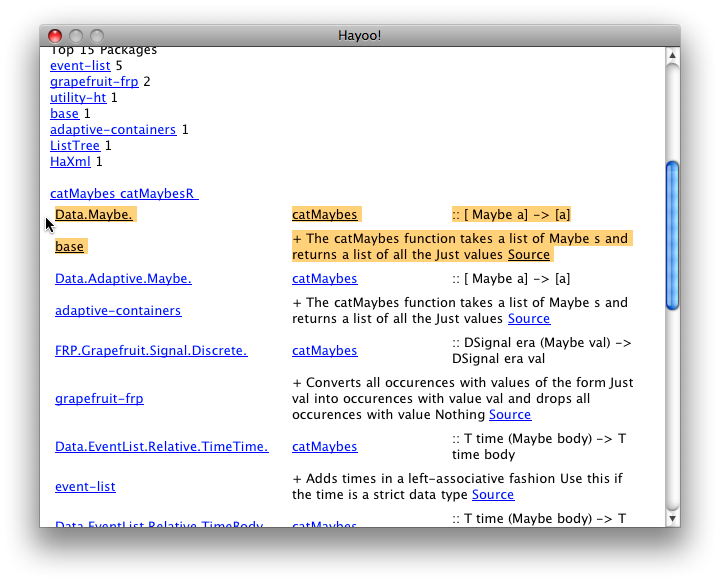
\includegraphics[width=.75\textwidth]{pictures/tut2/09}
		\caption{Tutorial 2 - \textsl{Jugando} contra \texttt{HFiaR.AI}}
		\label{tut210}
	\end{center}
\end{figure}
\paragraph{}Resta pues modificar la interfaz gr'afica para que permita al usuario jugar contra la computadora, utilizando la funci'on \texttt{aiDropIn} en los turnos correspondientes a la m'aquina.  Para ello, F'atima abre el m'odulo \texttt{HFiaR.GUI} y realiza los cambios pertinentes.  Estos cambios puede realizarlos utilizando \hpage\ o cualquier otro editor, pues por la naturaleza ``imperativa'' del c'odigo a modificar, \hpage\ no representar'a un beneficio importante.  Por el mismo motivo, no los detallamos en este informe.  Para quien desee observarlos puede encontrarlos en \htmladdnormallink{la p'agina web del proyecto hfiar en github}{http://github.com/elbrujohalcon/hfiar/commit/88a59a61d3dff930a96a1a51ab1daff4fcac9ef8\#diff-2}~\cite{hfiar}
\paragraph{}El 'ultimo paso que F'atima debe realizar es incluir su nuevo m'odulo en la lista de m'odulos del ejecutable \textsl{hfiar} dentro del archivo \textbf{hfiar.cabal}.  Una vez hechas estas modificaciones, puede ejecutar los siguientes comandos y disfrutar de un partido de su juego favorito contra la computadora:
\lstset{language=sh, frame=single, tabsize=4}
\begin{center}\begin{lstlisting}
$ cabal configure --user
$ cabal build
$ cabal install
$ ~/.cabal/bin/hfiar &
\end{lstlisting}\end{center}

\newpage
\subsubsection{Conclusiones}
\paragraph{}A lo largo de este tutorial hemos podido ver c'omo utilizar \hpage\ para \textsl{comprender} c'odigo \haskell\ a trav'es de \textsl{micro-testing}.  Hemos visto tambi'en como, utilizando esa misma t'ecnica, podemos construir paso a paso m'odulos \haskell\ medianamente complejos.  Pudimos ver c'omo \hpage\ nos permite editar los m'odulos al tiempo que los testeamos, de modo de utilizar un 'unico aplicativo para ambas cosas y no necesitar recurrir a la consola.
\paragraph{}Hemos podido ver c'omo \hpage\ se encuentra integrado con \cabal\ para permitir cargar proyectos previamente configurados y evitar al desarrollador lidiar con el manejo de extensiones, carpetas y m'odulos manualmente.  Esto es una importante ventaja que ofrece \hpage\, dado que la mayor'ia de los proyectos desarrollados en \haskell\ se encuentran organizados en paquetes \cabal.
\paragraph{}Tambi'en hemos observado la forma gr'afica con la que \hpage\ describe y permite navegar los m'odulos cargados, sus funciones y sus estructuras de datos para luego utilizarlas en nuestro c'odigo.

\newpage
\section{Desarrollo - ?`C'omo se hizo \hpage?}
\subsection{Arquitectura General}
\begin{epigraphs}
	\qitem{If you think good architecture is expensive, try bad architecture}{Brian Foote and Joseph Yoder}
\end{epigraphs}
\paragraph{}Las principales decisiones de arquitectura que se tomaron durante el desarrollo de \hpage\ tuvieron como principales motivaciones los siguientes requerimientos:
\begin{description}
\item[Conexi'on con GHC] \hpage\ deb'ia conectarse con el motor de GHC a trav'es de su API de modo de poder detectar e interpretar expresiones.  Para ello se utiliz'o \htmladdnormallink{hint}{http://projects.haskell.org/hint}~\cite{hint}
\item[Paralelismo] \hpage\ deb'ia permitir al usuario editar sus documentos mientras esperaba el resultado de la evaluaci'on de alguna expresi'on.  Para ello se cre'o \textsl{eprocess} y se implement'o un modelo de procesos utiliz'andolo.
\item[Errores Controlados] \hpage\ no deb'ia fallar si la evaluaci'on de una expresi'on fallaba.  M'as a'un, tambi'en deb'ia detectar posibles evaluaciones infinitas e informar estas situaciones al usuario
\item[Compatibilidad con GHCi] \hpage\ deb'ia ser capaz de reemplazar a \textsl{GHCi} y, por lo tanto, brindar toda las funcionalidades que esta aplicaci'on brinda.  En particular, deb'ia:
	\begin{itemize}
		\item ser multiplataforma
		\item detectar expresiones sint'acticamente inv'alidas
		\item identificar el tipo de cualquier expresi'on sint'acticamente v'alida
		\item identificar la clase de cualquier tipo sint'acticamente v'alido
		\item interpretar expresiones de cualquier tipo que sea instancia de la clase \textbf{Show}
		\item ejecutar e imprimir el resultado de expresiones de tipo \textbf{Show a $\Rightarrow$ IO a}
	\end{itemize}
\end{description}
\begin{figure}[hp]
	\begin{center}
        	\fbox{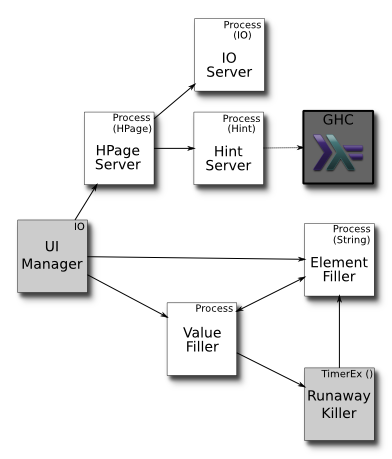
\includegraphics{pictures/architecture}}
		\caption{Arquitectura de \hpage}
		\label{arq1}
	\end{center}
\end{figure}
\subparagraph{}Teniendo en cuenta estos requerimientos, la arquitectura resultante puede ser descripta con el diagrama de la figura \ref{arq1}.  Esta figura presenta el estado del sistema en un instante dado.  Cada bloque representan un proceso o ``thread'' en ejecuci'on.  Cada uno de estos procesos se ejecuta dentro del entorno de una m'onada, la cual se encuentra identificada en la esquina superior derecha del bloque.  En el diagrama podemos identificar los siguientes componentes:
\begin{description}
	\item[UI Manager] Este es el thread que inicia el programa, genera y administra la interfaz del usuario utilizando las herramientas provistas por \textsl{wxHaskell}.  En este thread se mantiene el estado visual de la aplicaci'on: el estado de los controles, la 'ultima b'usqueda realizada, etc.
	\item[HPage Server] Este proceso, iniciado por el \textbf{UI Manager}, es el que comunica a la interfaz del usuario con la m'aquina virtual de GHC, a trav'es del \textbf{Hint Server}, captura sus errores y lo reinicia en caso de ser necesario.  En el caso de expresiones de tipo \textbf{IO a}, este mismo proceso se comunica con el \textbf{IO Server} para ejecutarlas y obtener su resultado o capturar sus errores.  En este proceso se mantiene el estado general de la aplicaci'on: sus p'aginas, expresiones, paquetes y m'odulos cargados, etc.
	\item[IO Server]Este proceso, iniciado por el  \textbf{HPage Server}, es el encargado de ejecutar acciones de tipo \textbf{IO a} en un entorno controlado y obtener su resultado.
	\item[Hint Server] Este proceso, iniciado por el \textbf{HPage Server}, mantiene una conexi'on con la m'aquina virtual de GHC (a la cual se muestra en la figura conectado a trav'es de una l'inea de puntos)
	\item[Char Filler] Este proceso, iniciado por el \textbf{UI Manager} cumple una muy sencilla funci'on: utilizando los procedimientos de env'io y recepci'on de mensajes provistos por \textsl{eprocess}, espera recibir un caracter (o sea, una expresi'on de tipo Char), para luego evaluarlo y enviar como respuesta su valor en forma normal.
	\item[Value Filler] Este proceso, iniciado por el \textbf{UI Manager} es el encargado de procesar el resultado obtenido del \textbf{HPage Server}.  Cabe recordar aqu'i que \haskell\ trabaja con evaluaci'on ``lazy'', por lo cual el resultado obtenido no ha sido a'un completamente procesado.  El \textbf{Value Filler} espera recibir un resultado y, al recibirlo, se encarga de evaluarlo y mostrarlo por pantalla, para ello env'ia y recibe mensajes del \textbf{Char Filler} a fin de procesar cada caracter a mostrar.
	\item[Runaway Killer] Este thread, creado utilizando la clase \textsl{TimerEx} provista por \textsl{wxHaskell}, es iniciado por cada \textbf{Value Filler} al momento de enviar un nuevo caracter al \textbf{Char Filler}.  El objetivo del \textbf{Runaway Killer} es el de detectar procesamiento ``posiblemente'' infinito.  B'asicamente, pasado un segundo de procesamiento, reinicia el \textbf{Char Filler} e informa al \textbf{Value Filler} que lo inici'o que el caracter que se esperaba procesar ha demorado demasiado y podr'ia desencadenar una evaluaci'on infinita.
\end{description}
\paragraph{}Para un mayor detalle, la figura \ref{seq1} nos muestra un diagrama de secuencia correspondiente a un proceso de evaluaci'on.  Para poder brindar un ejemplo completo, hemos ``fabricado'' un tipo que responde al siguiente c'odigo:
\lstset{language=haskell, frame=single, tabsize=4}
\begin{center}\begin{lstlisting}
data WithIfiniteChar = WIC

instance Show WithIfiniteChar where
    show WIC = ['c', head . show $ length [1..]]
\end{lstlisting}\end{center}
\subparagraph{}Como puede observarse, al intentar mostrar la expresi'on \texttt{WIC}, \hpage\ se encontrar'a con una cadena cuyo segundo caracter no puede computar pues requiere un c'alculo infinito, en la figura representamos este caracter con la letra $\Omega$.  All'i es donde entra en acci'on el \textbf{Runaway Killer} para informar esta situaci'on al usuario.
\begin{figure}[hp]
	\begin{center}
        	\fbox{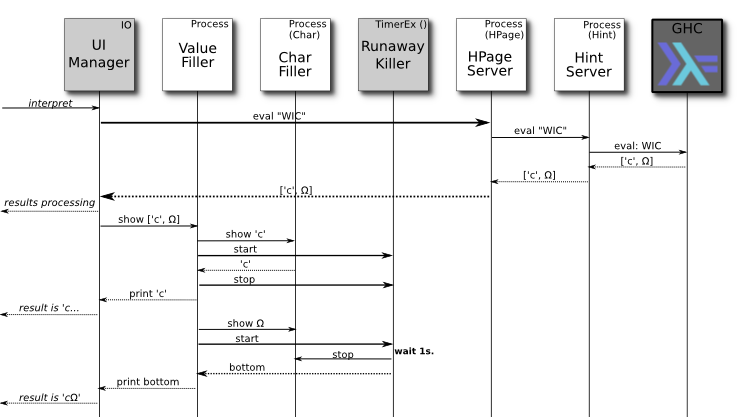
\includegraphics[width=\textwidth]{pictures/sequence}}
		\caption{Secuencia de Evaluaci'on de ``WIC''}
		\label{seq1}
	\end{center}
\end{figure}

\newpage
\subsection{Dise'no}
\begin{epigraphs}
	\qitem{Design and programming are human activities; forget that and all is lost}{Bjarne Stroustrup}
\end{epigraphs}
\paragraph{}Presentaremos a continuaci'on las principales decisiones de dise'no que se han tomado durante la creaci'on de \hpage.  Todas ellas tienen como fundamento los requerimientos principales exhibidos en la secci'on anterior y tambi'en algunos requerimientos adicionales, como la integraci'on con \cabal\ y \textsl{Hayoo!}.
\subsubsection{Concurrencia}
\paragraph{}Como hemos visto en la secci'on anterior, al momento de dise'nar \hpage\ tuvimos que considerar la necesidad de paralelizar tareas, para permitir al usuario, por ejemplo, trabajar en un documento mientras el motor de \hpage\ eval'ua una expresi'on.  Tambi'en debemos considerar que estas tareas a realizar en paralelo no son totalmente independientes sino que requieren una sincronizaci'on.  Tomando la idea del modo en que est'a dise'nado el lenguaje de programaci'on \textsl{Erlang}, decidimos implementar el paralelismo utilizando lo que denominamos \textsl{procesos}.  Conceptualmente, los \textsl{procesos} son hilos de ejecuci'on que se realizan en paralelo y pueden recibir o enviar mensajes.   Esta caracter'istica de mensajer'ia entre procesos es la que permite la sincron'ia cuando es necesaria.  Por otra parte, a diferencia de \textsl{Erlang}, al utilizar \haskell, los mensajes enviados de un proceso a otro pueden ser mucho m'as complejos.  Gracias al uso de m'onadas, un proceso puede enviar a otro directamente las acciones que desea que 'este ejecute, tal como deben ser ejecutadas.  Esta es una caracter'istica esencial para reducir la complejidad de la implementaci'on de todos nuestros procesos, en particular de aquellos que act'uan como servidores (\textbf{IO Server}, \textbf{HPage Server} y \textbf{Hint Server}), como veremos luego en la secci'on \textsl{Implementaci'on}.
\subsubsection{Bottoms}
\paragraph{}El lenguaje \haskell\ tiene una caracter'istica 'unica: \textsl{la evaluaci'on perezosa} o \textsl{lazy evaluation}.  Gracias a esta caracter'istica, las expresiones \haskell\ no son completamente evaluadas (reducidas a forma normal) hasta el momento en que realmente se necesita conocer su valor.  Dado que \hpage\ presenta al usuario un interprete de expresiones, es necesario que est'e preparado para no s'olo soportar sino tambi'en aprovechar esta caracter'istica.  En particular, dentro de \hpage\ las expresiones son reducidas a forma normal al momento de intentar mostrar el resultado de su evaluaci'on al usuario.  En ese momento, lo 'unico que se sabe es que la expresi'on a mostrar es de clase \textsl{Show}, lo que quiere decir que la misma es de tipo \texttt{[Char]}.  \hpage\ intenta entonces evaluar la expresi'on a mostrar y pueden suceder varias cosas:
\begin{itemize}
	\item Por supuesto, puede suceder que al evaluar la expresi'on se obtenga una cadena de caracteres, en cuyo caso \hpage\ simplemente presentar'a el resultado al usuario
	\item Puede suceder que, intentando evaluar la expresi'on se obtenga una cadena de caracteres de longitud infinita.  La pol'itica de \hpage\ en este caso es permitir al usuario decidir cu'ando desea abortar la evaluaci'on y mostrar la porci'on del resultado obtenida hasta ese momento
	\item Puede suceder tambi'en que, intentando evaluar un caracter, se genere un c'alculo ``infinito'' o una excepci'on.  En este caso tambi'en, \hpage\ permite al usuario cancelar la evaluaci'on cuando lo considere apropiado.
	\item Otra posibilidad es que, luego de presentar un caracter, al intentar obtener el resto de la cadena, \hpage\ encuentre un c'alculo ``infinito'' o una excepci'on.  En estos casos, se informa la situaci'on al usuario y se aborta la evaluaci'on de la expresi'on.
\end{itemize}
\subsubsection{Integraci'on}
\paragraph{}Una de las herramientas m'as comunmente usada por los desarrolladores haskell es \cabal.  \cabal\ (Common Architecture for Building Applications and Libraries) es una API distribuida con GHC que permite a un desarrollador agrupar f'acilmente un conjunto de m'odulos para producir un paquete. Es el sistema de compilaci'on est'andar para las aplicaciones y librer'ias de \haskell.  En un \textsl{paquete Cabal}, el desarrollador define los m'odulos que componen su aplicaci'on o librer'ia, los lugares (carpetas) donde encontrar el c'odigo fuente y los recursos que 'estos necesitan para funcionar, junto con las extensiones que se requieren para poder compilarlos.
\subparagraph{}\hpage\ por su parte, permite al desarrollador cargar o importar m'odulos para poder utilizarlos al momento de evaluar expresiones.  Tambi'en permite definir los lugares donde el compilador puede encontrar archivos fuentes y las extensiones que 'este debe utilizar al momento de compilar los archivos encontrados.
\subparagraph{}Observando estas similitudes, una integraci'on con \cabal\ es algo que surge de manera natural y \hpage\ lo provee.  \hpage\ permite al desarrollador cargar un paquete \cabal\ previamente configurado y de ese modo utilizar los m'odulos, extensiones y ubicaciones en 'el definidos.
\paragraph{}Otra herramienta, quiz'a no tan popular como \cabal, pero tambi'en muy 'util es \textsl{Hayoo!}.  \textsl{Hayoo!} es un motor de b'usqueda especializado en la documentaci'on de la API de \haskell.  El objetivo de \textsl{Hayoo!} es proporcionar una interfaz de b'usqueda interactiva y f'acil de usar para la documentaci'on de varios paquetes y librer'ias \haskell.  Conociendo esta herramienta, decidimos integrarla con \hpage\ de modo que el desarrollador pueda realizar consultas en su base de datos para obtener informaci'on sobre alguna funci'on, tipo, m'odulo, clase o expresi'on que desee analizar.

\subsection{Implementaci'on}
\begin{epigraphs}
	\qitem{Nothing resolves design issues like an implementation}{J. D. Horton}
	\qitem{A child of five would understand this. Send someone to fetch a child of five}{Groucho Marx}
\end{epigraphs}

\subsubsection{eprocess}
\paragraph{}Para la implementaci'on de \textsl{eprocess}, nuestra librer'ia de procesos, utilizamos dos herramientas de paralelismo y concurrencia que se encuentran muy bien descriptas en el libro \htmladdnormallink{Real World Haskell}{http://book.realworldhaskell.org/read/concurrent-and-multicore-programming.html}~\cite{realworldhaskell}.  Utilizamos \textsl{Threads} para paralelizar procesos y \textsl{Channels} y \textsl{MVars} para permitirles comunicarse.  Definimos entonces un tipo mon'adico para representar a las acciones a realizarse en procesos paralelos de tipo \texttt{m}, tales que retornan expresiones de tipo \texttt{a} y pueden recibir elementos de tipo \texttt{r}:
\begin{center}\begin{lstlisting}
newtype ReceiverT r m a = RT { internalReader :: ReaderT (Handle r) m a }
    deriving (Monad, MonadIO, MonadTrans, MonadCatchIO)
\end{lstlisting}\end{center}
\subparagraph{}Individualizamos luego este tipo gen'erico, definiendo el tipo \texttt{Process}:
\begin{center}\begin{lstlisting}
type Process r = ReceiverT r IO
\end{lstlisting}\end{center}
\subparagraph{}Finalmente definimos las funciones que permiten la ejecuci'on y mensajer'ia entre procesos:
\begin{center}\begin{lstlisting}
spawn :: MonadIO m => Process r k -> m (Handle r)
kill :: MonadIO m => Handle a -> m ()
self :: Monad m => ReceiverT r m (Handle r)
sendTo :: MonadIO m => Handle a -> a -> m ()
recv :: MonadIO m => ReceiverT r m r
\end{lstlisting}\end{center}
\subparagraph{}Las funciones \texttt{spawn} y \texttt{kill} inician y dentienen un proceso respectivamente.  \texttt{spawn} retorna como resultado un \texttt{Handle}, que identifica un'ivocamente al proceso y permite enviarle mensajes utilizando la funci'on \texttt{sendTo}.  Cabe notar que esta funci'on no necesita ser utilizada dentro de un \textsl{process} sino simplemente en cualquier instancia de la clase \texttt{MonadIO}.  De este modo, el \textsl{thread} que haya ejecutado \texttt{spawn} puede ejecutar \texttt{sendTo} para enviar mensajes al proceso que ha iniciado.
\subparagraph{}Luego, dentro de una instancia de \texttt{ReceiverT} se puede utilizar la funci'on \texttt{self} para conocer el propio \texttt{Handle} y \texttt{recv} para recibir mensajes.  Cabe notar que \texttt{recv} se ejecuta de manera bloqueante, emulando el comportamiento de la funci'on \texttt{receive} de \textsl{Erlang}.

\newpage
\subsubsection{Servers}
\paragraph{}Con el objetivo de separar la interacci'on con GHC del resto de la ejecuci'on del sistema y de esta manera, poder capturar sus excepciones y aislarlas, hemos encapsulado la ejecuci'on de estas acciones (correspondientes a la m'onada \texttt{Interpreter}) en un proceso particular, al que denominamos \textbf{Hint Server}.  Por otra parte, con objetivos similares, decidimos aislar la ejecuci'on de las acciones propias de \hpage\ (correspondientes a la m'onada \texttt{HPage}) de las relativas a la interfaz de usuario, para lo cual creamos el proceso \textbf{HPage Server}.  A su vez, tambi'en fue necesario ejeuctar acciones de la m'onada \texttt{IO} en un contexto controlado, por lo que desarrolamos el proceso \textbf{IO Server}.  Gracias al uso de m'onadas y los mecanismos provistos por \textsl{eprocess}, pudimos construir 'estos servers de una manera sencilla.   Mostramos, a modo de ejemplo e incluyendo comentarios explicativos, el c'odigo m'as significativo de uno de ellos:
\begin{center}\begin{lstlisting}
-- Para comenzar definimos un tipo ``ServerHandle'', que debe ser utilizado para
-- enviarle mensajes al servidor
newtype ServerHandle = SH {handle :: Handle (InterpreterT IO ())}

-- Convertimos a (ReceiverT r m) en una instancia de MonadInterpreter para poder
-- ejecutar las acciones que esperamos recibir como mensajes
instance MonadInterpreter m => MonadInterpreter (ReceiverT r m) where
    fromSession = lift . fromSession
    modifySessionRef a = lift . (modifySessionRef a)
    runGhc = lift . runGhc 

-- Definimos una funcion que inicia el servidor y retorna su handle
-- El servidor simplemente recibe acciones de tipo MonadInterpreter
-- y las ejecuta utilizando la funcion lift
start :: IO ServerHandle
start = (spawn $ makeProcess runInterpreter interpreter) >>= return . SH
    where interpreter =
            do
                setImports ["Prelude"]
                forever $ recv >>= lift

-- Definimos una funcion para ejecutar acciones asincronicamente
-- Esta funcion recibe la acciona a ejecutar junto con el handle del servidor
-- y devuelve una MVar que llenara con el resultado de la accion
asyncRunIn :: ServerHandle -> InterpreterT IO a
     -> IO (MVar (Either InterpreterError a))
asyncRunIn server action = do
     resVar <- liftIO newEmptyMVar
     sendTo (handle server) $ try action >>= liftIO . putMVar resVar
     return resVar

-- Definimos tambien una funcion para ejecutar resultados sincronicamente
-- Esta funcion envia al servidor la acciona a ejecutar y espera recibir el 
-- resultado para luego devolverlo
runIn :: ServerHandle -> InterpreterT IO a
       -> IO (Either InterpreterError a)
runIn server action = runHere $ do
     me <- self
     sendTo (handle server) $ try action >>= sendTo me
     recv

-- Finalmente, definimos una funcion que detiene al servidor utilizando la
-- la funcion kill
stop :: ServerHandle -> IO ()
stop = kill . handle
\end{lstlisting}\end{center}
\subparagraph{}Cabe destacar la simpleza de este m'odulo que, con no m'as de 25 l'ineas de c'odigo es capaz de ejecutar todas las acciones que provee \textsl{hint} en un proceso aislado y controlado.

\subsubsection{M'odulos de \hpage}
\paragraph{}El m'odulo principal de la aplicaci'on es el denominado \texttt{HPage.Control}.  Este m'odulo describe la m'onada \texttt{HPage} e incluye todas las acciones que pueden realizarse en ella.  Es el encargado de mantener el estado del sistema, para lo cual hemos definido un tipo de datos llamado \texttt{Context}, que mostraremos a continuaci'on.
\subparagraph{} Los principales componentes del estado del sistema son:
\begin{description}
	\item[activePackage] El paquete \cabal\ activo, si es que se ha cargado alguno.
	\item[pages] Las p'aginas que el usuario est'a viendo.  Cabe notar que un usuario puede tener varias p'aginas activas a la vez, una con cada documento.
	\item[loadedModules / importedModules] Los m'odulos que el usuario ha cargado / importado
	\item[server] El handle del \textbf{Hint Server} que el mismo \textbf{HPage Server} inicia y mantiene
	\item[ioServer] El handle del \textbf{IO Server} que el mismo \textbf{HPage Server} inicia y mantiene
	\item[running] La acci'on que se encuentra ejecut'andose de manera asincr'onica, si es que hay alguna
	\item[recoveryLog] El log de acciones realizadas hasta el momento, 'util al momento de detener el \textbf{Hint Server}
\end{description}
\begin{center}\begin{lstlisting}
newtype Expression = Exp {exprText :: String}       
    deriving (Eq, Show)

data InFlightData = LoadModules { loadingModules :: Set String,
                                  runningAction :: Hint.InterpreterT IO ()
                                  } |
                    ImportModules { importingModules :: Set String,
                                    runningAction :: Hint.InterpreterT IO ()
                                    } | 
                    SetSourceDirs { settingSrcDirs :: [FilePath],
                                    runningAction :: Hint.InterpreterT IO ()
                                    } |
                    SetGhcOpts { settingGhcOpts :: String,
                                 runningAction :: Hint.InterpreterT IO ()
                                 } |
                    Reset

data Page = Page { -- Display --
                   expressions :: [Expression],
                   currentExpr :: Int,
                   undoActions :: [HPage ()],
                   redoActions :: [HPage ()],
                   -- File System --
                   original :: [Expression],
                   filePath    :: Maybe FilePath
                  }
                  
data Context = Context { -- Package --
                         activePackage :: Maybe PackageIdentifier,
                         pkgModules :: [Hint.ModuleName],
                         -- Pages --
                         pages :: [Page],
                         currentPage :: Int,
                         -- GHC State --
                         loadedModules :: Set String,
                         importedModules :: Set String,
                         extraSrcDirs :: [FilePath],
                         ghcOptions :: String,
                         server :: HS.ServerHandle,
                         ioServer :: HPIO.ServerHandle,
                         -- Actions --
                         running :: Maybe InFlightData,
                         recoveryLog :: Hint.InterpreterT IO ()
                       }
\end{lstlisting}\end{center}
\subparagraph{}Notese que el paquete \cabal, las extensiones y los m'odulos cargados o importados, etc. son independientes de las p'aginas con las que el usuario est'e trabajando, por lo que el usuario por ejemplo no puede manejar dos paquetes \cabal\ a la vez.  'Esto se debe a que la API de \textsl{GHC} no permite la utilizaci'on de \textsl{multi-threading}, por lo tanto, dentro de un programa s'olo puede haber una 'unica lista de m'odulos cargados/importados, una 'unica lista de extensiones, etc.
\subparagraph{}Tambi'en debe notarse que mucha de la informaci'on de estado guardada en el \texttt{Context} es ``redundante'' pues se configura directamente en el \textbf{Hint Server}.  Eso se debe a que ante la eventual ca'ida del \textbf{Hint Server}, el \textbf{HPage Server} lo reinicia y restaura su estado utilizando esos datos.
\subparagraph{}Finalmente, \texttt{running} y \texttt{recoveryLog} se utilizan para permitir al usuario cancelar acciones que intenta ejecutar.  Cada acci'on que se desea realizar de forma asincr'onica, devuelve una \textsl{MVar} que se llenar'a en caso de finalizar la acci'on con 'exito y se acumular'a en el \texttt{recoveryLog}.  En caso de cancelar, el \textbf{HPage Server} reinicia al \textbf{IO Server} y al \textbf{Hint Server}, configura a este 'ultimo seg'un los dem'as par'ametros (ej: \texttt{ghcOptions}) y vuelve a ejecutar el \texttt{recoveryLog} para ``ponerlo al d'ia''.
\subparagraph{}El estado de las p'aginas con las que el usuario trabaja est'a definido como una lista de expresiones y dos listas de acciones para permitir el uso de \textsl{undo} y \textsl{redo}.  Finalmente, si la p'agina corresponde a un archivo en disco, \hpage\ identifica el ``path'' del mismo para poder guardarlo o recargarlo de ser necesario.
\subparagraph{}Gracias a haber separado la l'ogica correspondiente a la interfaz de usuario y la propia de \hpage, hemos podido desarrollar esta 'ultima utilizando la t'ecnica de TDD (Test Driven Development) ~\cite{tdd}.  Para ello utilizamos \htmladdnormallink{QuickCheck}{http://www.cs.chalmers.se/~rjmh/QuickCheck/}~\cite{quickcheck}, una herramienta que nos permiti'o ir desarrollando y verificando tests de manera incremental hasta alcanzar la actual definici'on del \textbf{HPage Server}.  Los tests desarrollados pueden ser ejecutados utilizando el siguiente comando:
\lstset{language=sh, frame=single, tabsize=2}
\begin{center}\begin{lstlisting}
$ cabal test hpage
\end{lstlisting}\end{center}
\lstset{language=haskell, frame=single, tabsize=4}

\subsubsection{UI}
\paragraph{}La interfaz gr'afica de \hpage\ est'a desarrollada utilizando \textsl{wxHaskell}, un framework elegido por ser multi-plataforma y, gracias a estar constru'ido sobre \textsl{wxWidgets}, presentar un ``look\&feel'' nativo en distintos entornos.  \textsl{wxHaskell} es un framework sencillo para utilizar y entender y, pese a que a'un se encuentra en per'iodo de evoluci'on, es suficientemente estable.  Sin embargo, tal como puede verse en \textsl{wxhNotepad} hemos tenido que superar varios escollos hasta lograr una UI estable e intuitiva.  A los lectores interesados en estos detalles t'ecnicos les recomendamos los art'iculos escritos por Jeremy O'Donoghue en su tutorial \htmladdnormallink{Building a text editor}{http://wewantarock.wordpress.com/2010/01/31/building-a-text-editor-part-1/}~\cite{wewantarock}.

\newpage
\section{Resultados}
\subsection{Objetivos Alcanzados}
\begin{epigraphs}
	\qitem{Results! Why, man? I have gotten a lot of results. I know several thousand things that wont work}{Thomas A. Edison}
	\qitem{Kids, you tried your best and you failed miserably. The lesson is: ``never try''}{Homer Simpsons}
\end{epigraphs}
\paragraph{}A primera vista, \hpage\ puede parecer simplemente un editor de texto al que se le agrega la posibilidad de interpretar expresiones \haskell.  Esta visi'on es cierta, y en s'i misma es un avance con respecto a las herramientas ya existentes pues permite intercalar en un mismo documento texto libre y expresiones \haskell.
\subparagraph{}Sin embargo, \hpage\ presenta varios atributos que generan un importante valor agregado:
\begin{itemize}
	\item Permite configurar el entorno manual o autom'aticamente en base a un paquete \cabal
	\item Permite buscar documentaci'on sobre expresiones \haskell\ utilizando \textsl{Hayoo!}
	\item Permite al usuario editar texto mientras espera el resultado de la evaluaci'on de una expresi'on
	\item Permite visualizar y analizar expresiones que contengan errores, ``bottoms'' o que generen c'alculos ``infinitos''
\end{itemize}
\subparagraph{}Son todas estas caracter'isticas las que convierten a \hpage\ en una herramienta de gran utilidad para todo desarrollador \haskell, desde el estudiante universitario que generalmente se encuentra frente a la necesidad de ``entender''  funciones del lenguaje y as'i aprenderlo hasta el desarrollador avanzado que necesita debuggear sus aplicaciones.

\newpage
\subsection{Trabajo a Realizar}
\begin{epigraphs}
	\qitem{Inside every large program, there is a small program trying to get out}{C.A.R. Hoare}
	\qitem{I'm a man with a one-track mind, so much to do in one life-time}{Queen}
\end{epigraphs}
\paragraph{}\hpage\ es todav'ia una aplicaci'on en desarrollo y de c'odigo abierto.  A'un queda mucho por hacer y por eso la hemos publicado en internet utilizando \htmladdnormallink{github}{http://github.com}~\cite{github}.  Gracias a este servicio, se encuentra habilitada \htmladdnormallink{una lista de bugs y sugerencias}{http://github.com/elbrujohalcon/hPage/issues} en constante actualizaci'on.  Entre las tareas que all'i se encuentran al d'ia de hoy, cabe destacar:
\begin{description}
	\item[ByteStrings] Las aplicaciones \haskell\ tradicionales manejan el texto utilizando \textbf{Strings} (o sea, listas de caracteres), pero ya se encuentra a disposici'on del desarrollador \haskell\ una nueva herramienta que permite manejar texto de una manera m'as 'optima: \textbf{ByteStrings}.  \hpage\ utiliza en su mayor'ia \textbf{Strings} y podr'ia ser optimizado migrando la mayor cantidad posible a \textbf{ByteStrings}.
	\item[Mejoras Visuales] La UI de \hpage\ tiene mucho por mejorar y optimizar.  Ejemplos de esto son el coloreo de c'odigo y la autocompleci'on.  \textsl{wxHaskell} se encuentra en constante desarrollo y sus optimizaciones deber'ian ser aprovechadas por \hpage\ cuando sea posible.
	\item[\cabal] La actual integraci'on con \cabal\ cubre lo b'asico de la configuraci'on de paquetes, como las extensiones y los m'odulos, pero \cabal\ permite describir varias cosas m'as que podr'ian ser aprovechadas por \hpage\ como la ubicaci'on de librer'ias y otros archivos
	\item[Auto Reload] Una caracter'istica que ser'ia muy 'util agregar a \hpage\ es la recarga autom'atica de los m'odulos modificados.  De este modo, el desarrollador no necesitar'ia presionar el bot'on ``reload'' cada vez que modifica un m'odulo para que \hpage\ tome los cambios realizados.
\end{description}
\newpage
\section{Agradecimientos}
\paragraph{}Este proyecto nunca se podr'ia haber llevado a cabo sin la ayuda de muchas personas que contribuyeron de una u otra manera a su realizaci'on.  Entre ellas debemos agradecer especialmente a quienes nos han ayudado en la comprensi'on, \textbf{correcci'on} y manejo de \textsl{wxHaskell}: \htmladdnormallink{Arjan van IJzendoorn}{http://nl.linkedin.com/pub/arjan-van-ijzendoorn/5/ba8/480}, \htmladdnormallink{Eric Y. Kow}{mailto:eric.kow@gmail.com} y \htmladdnormallink{Jeremy O. Donoghue}{http://uk.linkedin.com/pub/jeremy-o-donoghue/4/7b/478}. Tambi'en queremos agradecer a \htmladdnormallink{Timo B. H\"ubel y Sebastian M. Schlat}{http://holumbus.fh-wedel.de/} que nos han permitido integrar \hpage\ con su herramienta \textsl{Hayoo!}.  Y no podr'iamos dejar de mencionar a nuestros ``beta-testers'': \htmladdnormallink{Abram Hindle}{http://softwareprocess.es/index.cgi/SoftwareProcess.es}, \htmladdnormallink{Mariano Perez Rodriguez}{mailto:mariano.perez.rodriguez@gmail.com}, \htmladdnormallink{Facundo Villanueva}{http://twitter.com/facuvillanueva}, \htmladdnormallink{Federico Grassi}{http://www.google.com/profiles/federico.grassi} y \htmladdnormallink{Bernab'e Panarello}{http://www.linkedin.com/pub/bernab'e-panarello/8/512/b48}.  Por 'ultimo, pero no por eso menos importante, queremos agradecer a \htmladdnormallink{Dar'io Ruellan}{http://www.google.com/profiles/dario.ruellan} quien ha creado nuestra \htmladdnormallink{p'agina web}{http://haskell.hpage.com}.
\paragraph{}Personalmente yo, \htmladdnormallink{Fernando Benavides}{http://google.com/profiles/greenmellon}, quisiera agradecer a mi mujer, Constanza Zappala, que me ha acompa'nado, ayudado y soportado durante el m'as de un a'no y medio que dur'o el desarrollo de este proyecto, a Juan Jos'e Comellas, Alejandro Tolomei, Francisco de Ezcurra y toda la gente de \htmladdnormallink{Novamens S.A.}{http://www.novamens.com}, la empresa en la que trabajo, por su inter'es y contribuci'on al proyecto, a todos los profesores de \textsl{Algor'itmos I} (Inclu'ida la Caja Vengadora) y \textsl{Paradigmas de Lenguajes de Programaci'on} por introducirme en el apasionante mundo de la programaci'on funcional y especialmente en \haskell, y por supuesto, a mis profesores Daniel Gor'in y Diego Garverbetsky, que desde el primer momento creyeron en m'i y en esta idea loca de ``hacer algo parecido a las cosas que tienen los que trabajan con objetos'' con la que llegu'e a aquella primera reuni'on con ellos.
\newpage
\bibliography{hpage}
\end{document}